\documentclass[10pt,twocolumn,letterpaper]{article}

\usepackage{iccv}
\usepackage{times}
\usepackage{epsfig}
\usepackage{graphicx}
\usepackage{amsmath}
\usepackage{amssymb}


\usepackage{color}
\usepackage{times}
\usepackage{overpic}
\usepackage{bm}
\usepackage{tabu}
\usepackage{bbding}
% \usepackage{multicol}
\usepackage{multirow}
% \usepackage{eso-pic}
% \usepackage{xcolor}
\usepackage[table]{xcolor}
% \usepackage[marginal]{footmisc}

% \documentclass[a4paper,x11names]{article}
% \usepackage{xcolor}
% \renewcommand{\thefootnote}{}#
% Include other packages here, before hyperref.

% If you comment hyperref and then uncomment it, you should delete
% egpaper.aux before re-running latex.  (Or just hit 'q' on the first latex
% run, let it finish, and you should be clear).
\usepackage[pagebackref=true,breaklinks=true,letterpaper=true,colorlinks,bookmarks=false]{hyperref}

\iccvfinalcopy % *** Uncomment this line for the final submission

\def\iccvPaperID{3649} % *** Enter the ICCV Paper ID here
\def\httilde{\mbox{\tt\raisebox{-.5ex}{\symbol{126}}}}

% Pages are numbered in submission mode, and unnumbered in camera-ready
\ificcvfinal\pagestyle{empty}\fi

\begin{document}

%%%%%%%%% TITLE
\title{Human-centric Scene Understanding for 3D Large-scale Scenarios}

\author{\textbf{
Yiteng Xu$^{1,}$\thanks{Equal contribution. $\dagger$ Corresponding author. This work was supported by NSFC (No.62206173), Natural Science Foundation of Shanghai (No.22dz1201900), MoE Key Laboratory of Intelligent Perception and Human-Machine Collaboration (ShanghaiTech University), Shanghai Frontiers Science Center of Human-centered Artificial Intelligence (ShangHAI), Shanghai Engineering Research Center of Intelligent Vision and Imaging.}  ,  
Peishan Cong$^{1,}\footnote[1]{}$  , 
Yichen Yao$^{1,}\footnote[1]{}$  ,}\\
\textbf{
Runnan Chen$^{2}$, 
Yuenan Hou$^{3}$, 
Xinge Zhu$^{4}$, 
Xuming He$^{1}$, 
Jingyi Yu$^{1}$, 
Yuexin Ma$^{1,}$\footnote[2]{}}\\ 
$^{1}$ ShanghaiTech University
$^{2}$ The University of Hong Kong \\
$^{3}$ Shanghai AI Laboratory 
$^{4}$ The Chinese University of Hong Kong\\
{\tt\small \{xuyt1,congpsh,yaoych,mayuexin\}@shanghaitech.edu.cn}}

\makeatletter
\let\@oldmaketitle\@maketitle% Store \@maketitle
\renewcommand{\@maketitle}{
   \@oldmaketitle% Update \@maketitle to insert...
 \begin{center}
     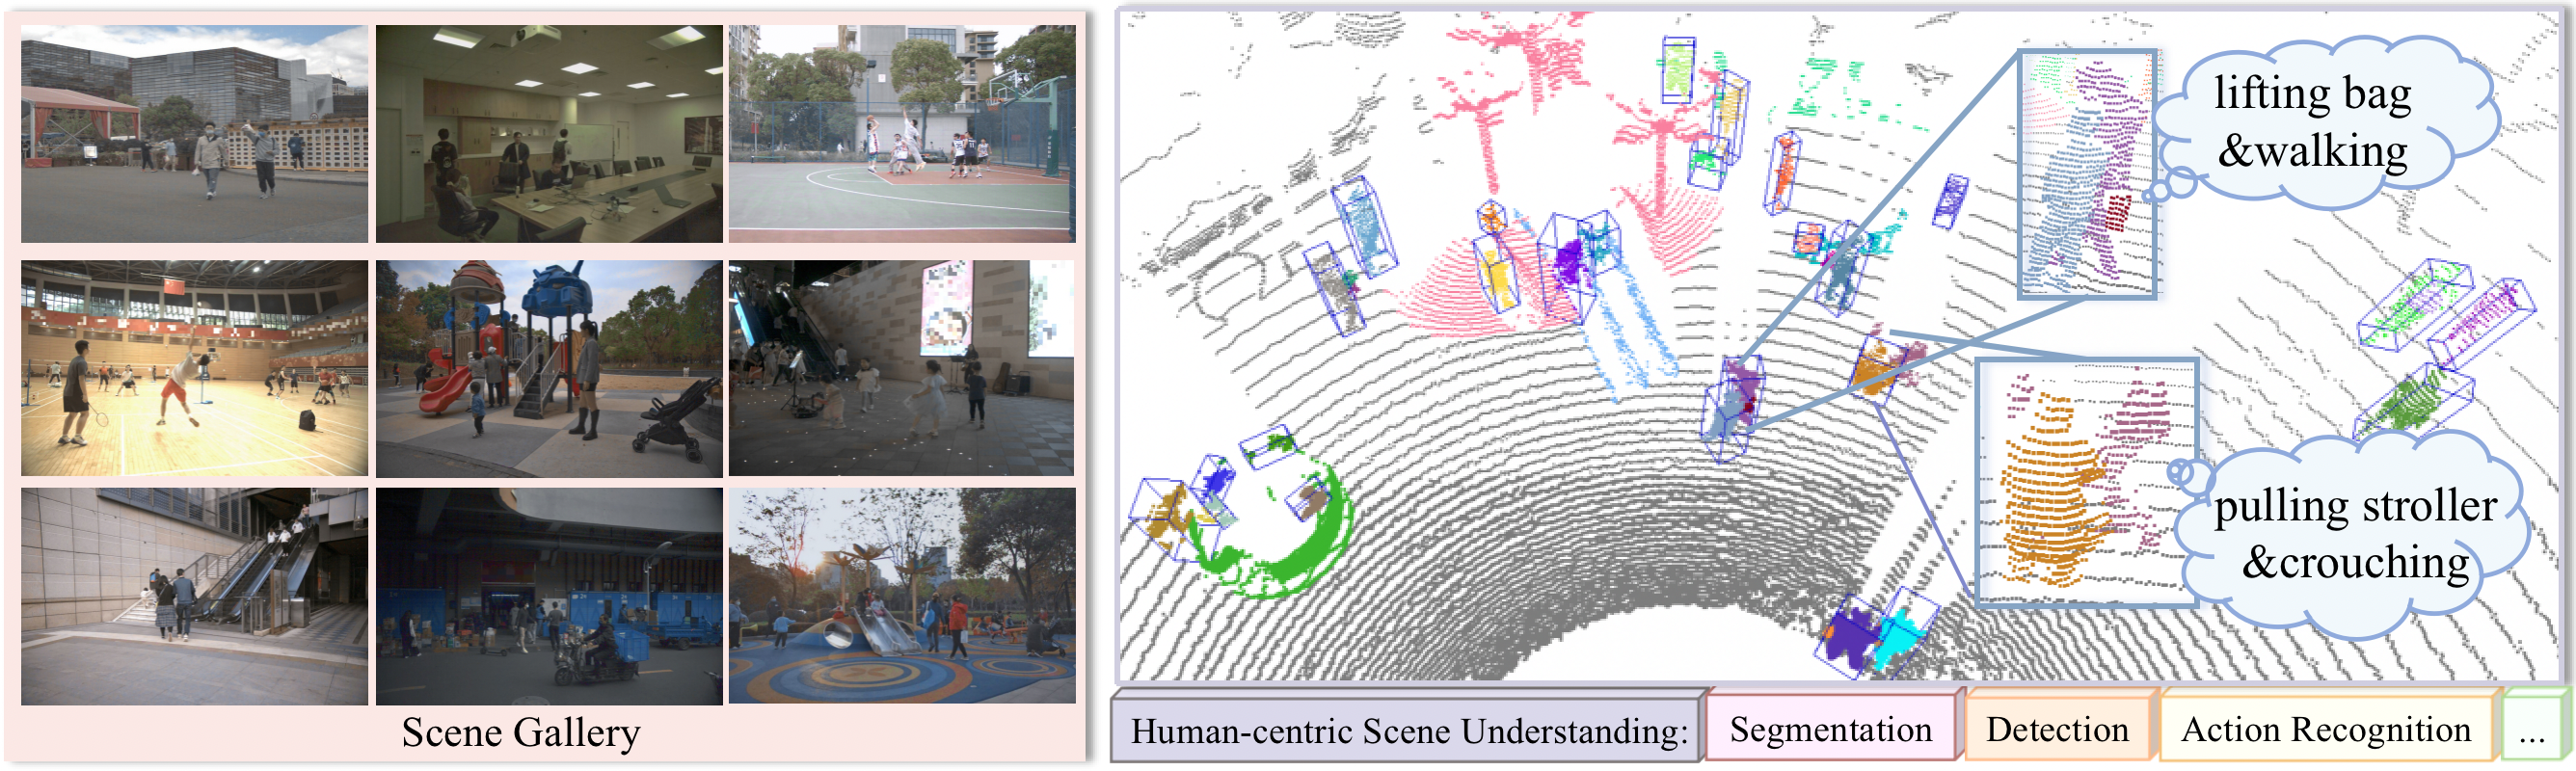
\includegraphics[width=2.1\columnwidth]{pic/teasor.png}
 \end{center}
   %\vspace{-1ex}
  \refstepcounter{figure}\normalfont Figure~\thefigure. 
  The left shows several scenes captured in HuCenLife, which covers diverse human-centric daily-life scenarios. The right demonstrates rich annotations of HuCenLife, which can benefit many tasks for 3D scene understanding .
  \label{fig:teaser}
  \newline
  }
\makeatother

\maketitle
% Remove page # from the first page of camera-ready.
\ificcvfinal\thispagestyle{empty}\fi


%%%%%%%%% ABSTRACT
\begin{abstract}

\input{sec/abstract}
\end{abstract}

%%%%%%%%% BODY TEXT
\section{Introduction}
\label{sec:intro}
\input{sec/intro}

%------------------------------------------------------------------------
\section{Related Work}
\label{sec:related}
\input{sec/related}
%-------------------------------------------------------------------------

\section{HuCenLife Dataset}
\label{sec:dataset}




\begin{table*}[ht]
\centering
\caption{Comparison with related datasets for 3D scene understanding. There are some abbreviations, where ``pc'' denotes LiDAR point cloud, ``ins. seg.'' means instance segmentation, ``bbx'' is bounding box, and ``inter. obj.'' denotes objects having interactions with humans.}
\label{tab:compare}
\resizebox{\linewidth}{!}{
\begin{tabular}{c|c|c|c|c|c|cc|ccc|cc}
\hline
      \rowcolor{blue!5}   Dataset     & Data   &  LiDAR & Point Cloud
&Person &Person &\multicolumn{2}{c|}{Scenes} &\multicolumn{3}{c|}{Annotation Content}& \multicolumn{2}{c}{Annotation Targets} \\ \cline{7-13}   

\rowcolor{blue!5} &Modality & Beam&Frame&Number&Per Frame& indoor & outdoor & ins. seg.& 3D bbx& action& multi-person& inter. obj.
\\\hline
ScanNet\cite{dai2017scannet}               &RGBD         & -  &-&-&-& \textcolor{green}{\Checkmark}& \textcolor{red}{\XSolidBrush}    &  \textcolor{green}{\Checkmark}       &    \textcolor{green}{\Checkmark}      & \textcolor{red}{\XSolidBrush}              & \textcolor{red}{\XSolidBrush}  & \textcolor{red}{\XSolidBrush}  \\\hline
S3DIS\cite{armeni20163d}&RGBD  
&-&-&-& -  & \textcolor{green}{\Checkmark}& \textcolor{red}{\XSolidBrush}    &  \textcolor{green}{\Checkmark}       &    \textcolor{green}{\Checkmark}      & \textcolor{red}{\XSolidBrush}              & \textcolor{red}{\XSolidBrush}  & \textcolor{red}{\XSolidBrush}  \\\hline
SUN RGB-D\cite{song2015sun}&RGBD&-
&-&-&-&\textcolor{green}{\Checkmark} &\textcolor{red}{\XSolidBrush}    & \textcolor{red}{\XSolidBrush}    &\textcolor{green}{\Checkmark}   & \textcolor{red}{\XSolidBrush}         &\textcolor{red}{\XSolidBrush}    & \textcolor{red}{\XSolidBrush}
\\\hline
NTU RGB+D\cite{shahroudy2016ntu}                &RGBD        &-  &-&-&-
&\textcolor{green}{\Checkmark} &\textcolor{red}{\XSolidBrush}    & \textcolor{red}{\XSolidBrush}       & \textcolor{red}{\XSolidBrush}       &\textcolor{green}{\Checkmark}  &\textcolor{red}{\XSolidBrush}    & \textcolor{red}{\XSolidBrush}     \\\hline

BEHAVE\cite{bhatnagar2022behave}          &RGBD       &-   &
15.8k& 15.8k&1
&\textcolor{green}{\Checkmark} &\textcolor{red}{\XSolidBrush}    &   \textcolor{green}{\Checkmark}     &  \textcolor{red}{\XSolidBrush}      & \textcolor{green}{\Checkmark}      &\textcolor{red}{\XSolidBrush}    &\textcolor{green}{\Checkmark}          \\\hline

SemanticKITTI\cite{behley2019semantickitti}      &pc      & 64 & 43k&9.7k&0.2&\textcolor{red}{\XSolidBrush}  & \textcolor{green}{\Checkmark} &   \textcolor{green}{\Checkmark}     &  \textcolor{red}{\XSolidBrush}         &\textcolor{red}{\XSolidBrush}  &    \textcolor{green}{\Checkmark}           & \textcolor{red}{\XSolidBrush}       \\\hline

KITTI\cite{geiger2012we}      &image\&pc      & 64 & 15k &4.5k&0.3&
\textcolor{red}{\XSolidBrush}  & \textcolor{green}{\Checkmark}  &  \textcolor{green}{\Checkmark} &   \textcolor{green}{\Checkmark}            &\textcolor{red}{\XSolidBrush}  &    \textcolor{green}{\Checkmark}           & \textcolor{red}{\XSolidBrush}       \\\hline


Waymo\cite{sun2020scalability}         &image\&pc   & 64 &  230k& 2.8M&12&
\textcolor{red}{\XSolidBrush}  & \textcolor{green}{\Checkmark}&   \textcolor{green}{\Checkmark}     &   \textcolor{green}{\Checkmark}     &\textcolor{red}{\XSolidBrush}  &    \textcolor{green}{\Checkmark}           & \textcolor{red}{\XSolidBrush}       \\\hline

nuScenes\cite{caesar2020nuscenes}         &image\&pc     & 32 & 40k &208k&5&\textcolor{red}{\XSolidBrush}  & \textcolor{green}{\Checkmark}&   \textcolor{green}{\Checkmark}     &   \textcolor{green}{\Checkmark}     &\textcolor{red}{\XSolidBrush}  &    \textcolor{green}{\Checkmark}           & \textcolor{red}{\XSolidBrush}       \\\hline

STCrowd\cite{cong2022stcrowd}           &image\&pc    & 128  & 11k &219k&20&\textcolor{red}{\XSolidBrush}  & \textcolor{green}{\Checkmark} & \textcolor{red}{\XSolidBrush}        & \textcolor{green}{\Checkmark}        & \textcolor{red}{\XSolidBrush}  &  \textcolor{green}{\Checkmark}        & \textcolor{red}{\XSolidBrush}         \\\hline


\textbf{HuCenLife}          &image\&pc      &128 & 6.1k& 65k&11&\textcolor{green}{\Checkmark}   & \textcolor{green}{\Checkmark}  & \textcolor{green}{\Checkmark}       & \textcolor{green}{\Checkmark}  & \textcolor{green}{\Checkmark} &  \textcolor{green}{\Checkmark} & \textcolor{green}{\Checkmark}  \\ \hline
\end{tabular}
}
\vspace{-2ex}
\end{table*}


HuCenLife is the first dataset that emphasizes human-centric 3D scene understanding, containing indoor and outdoor daily-life scenes with rich annotations of human activities, human-human interactions, and human-object interactions, which facilitates the development of intelligent security, assistive robots, human-machine cooperation, \etc.
%HuCenLife focuses on human-centric 3D scene understanding and captures diverse daily-life scenes, which contains rich human-human interactions and human-object interactions in large-scale indoor or outdoor scenarios. 
In this section, we first introduce the data acquisition in Sec.\ref{subsec:Acquisition}, and then provide important annotation statistics in Sec.\ref{subsec:Statistics}, and finally highlight the novelties of HuCenLife by comparing with existing influential datasets in Sec.\ref{subsec:Characteristic}.


\subsection{Data Acquisition}
\label{subsec:Acquisition}
To collect the dataset, we built a Visual-LiDAR Capture System, which mainly consists of one 128-beam Ouster-OS1 LiDAR and six industrial cameras in a circle, as Fig ~\ref{fig:sensor} shows. All sensors are tied in fixed positions on the bracket with mechanical synchronization. The LiDAR has a $360^{\circ}$ horizon field of view (FOV) $\times 45^{\circ}$ vertical FOV, and each camera has a $75^{\circ} \times 51.6^{\circ}$ FOV with $1920\times1200$ image resolution. For our equipment, LiDAR captures raw point cloud in $10$Hz and camera takes pictures in $32$Hz.



% \begin{figure}[t]
%     \centering
%     \includegraphics[width=1\columnwidth]{pic/dataset_scenes.png}
%     \caption{Diverse scenes in HuCenLife, containing indoor and outdoor large-scale scenarios in day and night with rich human activities, human-human interactions, and human-object interactions. }
%     \label{fig:dataset_scenes}
% \end{figure}

\begin{figure}[t]
    \centering
    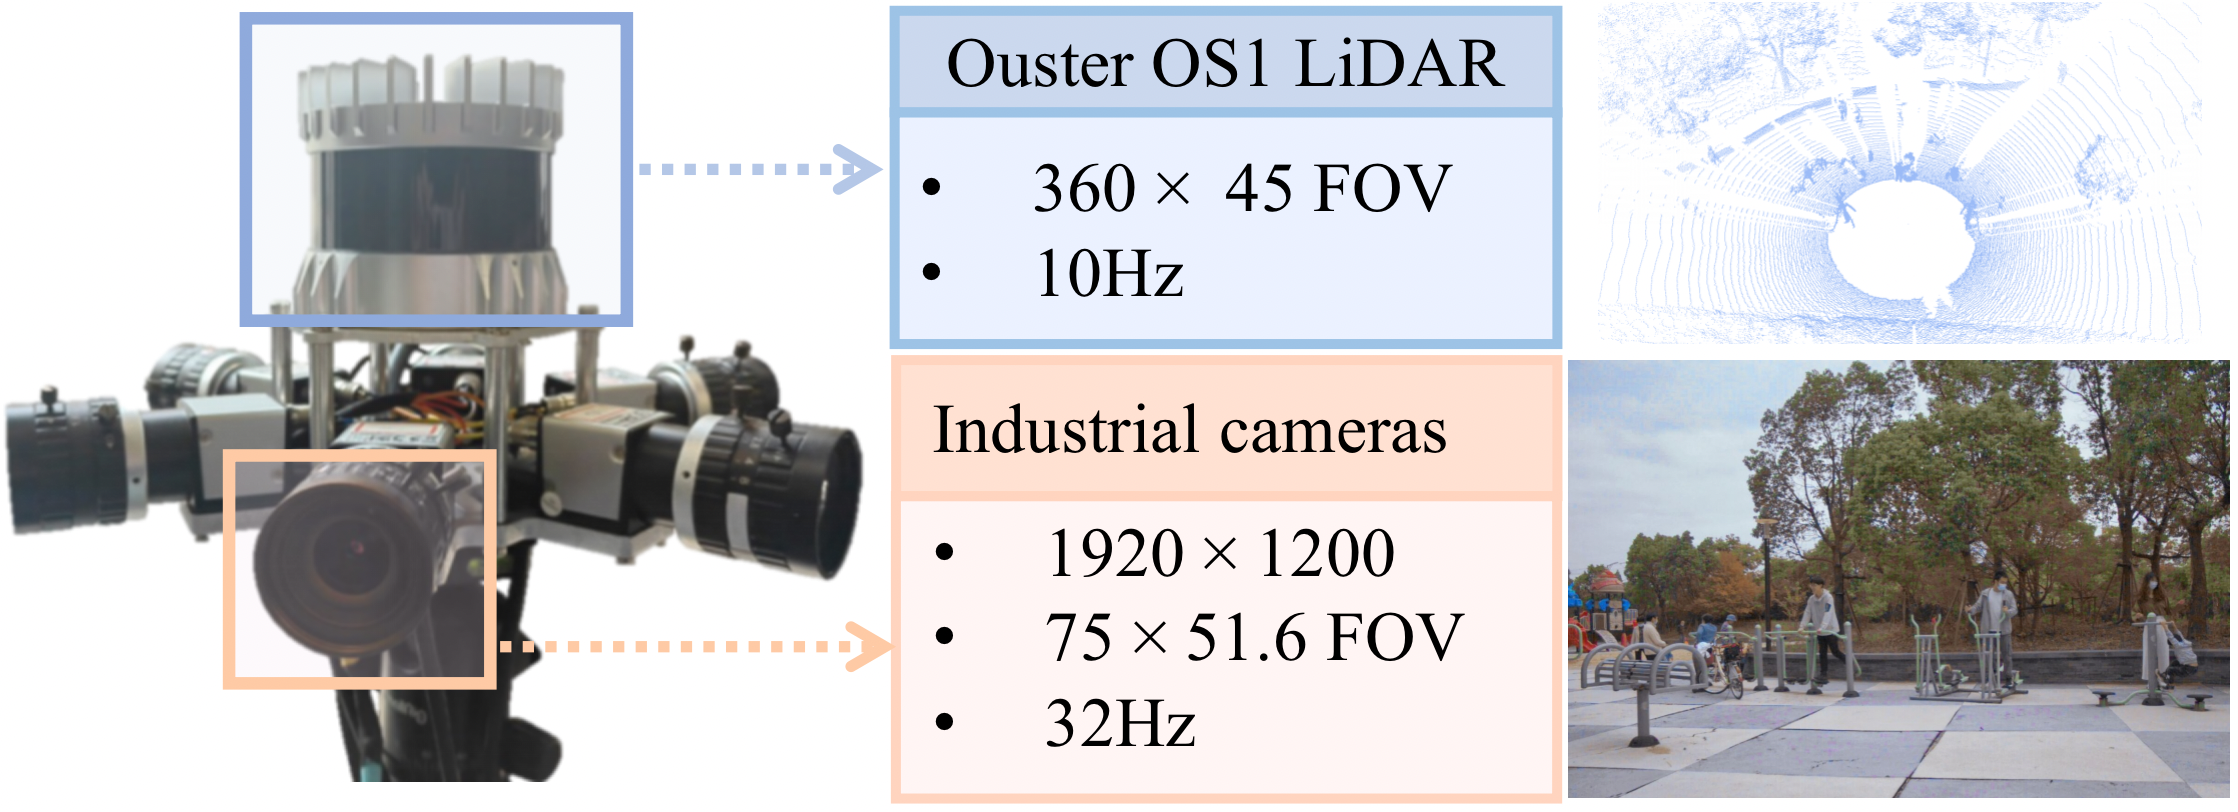
\includegraphics[width=1\columnwidth]{pic/sensor.png}
    \caption{Sensor setup for data collection. }
    \label{fig:sensor}
    \vspace{-2ex}
\end{figure}

\subsection{Annotation}
\label{subsec:Statistics}

We manually annotated all humans and these objects with interactions with humans in LiDAR point cloud by referring to the synchronized image. We select one frame per second for labeling and finally obtain $6,185$ frames ($103$ minutes) of annotated LiDAR point cloud. For each target, we provide four kinds of annotations, \ie, point cloud-based instance segmentation, 3D bounding box, human action classification, and tracking ID across consecutive frames, like Fig ~\ref{fig:teaser} shows. In HuCenLife, there are $65,265$ human instances in total, including $58,354$ adults and $6,911$ children, and $31,303$ human-interacted objects. There are $20$ categories of objects and $12$ kinds of human actions. Specifically, the HuCenLife dataset is collected in $15$ distinguished locations with $32$ human-centric daily-life scenes, including playground, shopping mall, campus, park, gym, meeting room, express station, \etc. For each scene, there are $11$ persons on average with multiple interacted objects, and for some complex scenes, there are about $70$ persons. The diverse density distributions in HuCenLife bring challenges for related research.
%Because the visual-LiDAR device is usually settled beside the scene to eliminate its affect on peoples' normal activities, we only annotate $180^{\circ}$ view of LiDAR point cloud and corresponding images of three cameras (where different scenes vary in cameras), which covers pertinent contents of scenes. 
More detailed annotation introductions are in the supplementary material.


\subsection{Characteristics}
\label{subsec:Characteristic}
We introduce the basic information of HuCenLife and compare it with related popular datasets in Table ~\ref{tab:compare}. In particular, we conclude four highlights of our dataset below.
%from five main aspects, including the modality of acquisition data, sensor configuration, data-collection scenes, annotation content, and annotation targets. In particular, we  

\textbf{Large-scale Dynamic Scenarios.} 
Benefiting from the long-range-sensing and light-independent properties of LiDAR, HuCenLife contains data of diverse large-scale scenes day and night. Unlike indoor datasets~\cite{dai2017scannet} where the scene is pre-scanned and has only static objects, HuCenLife provides online captured multi-modal visual data of dynamically changing scenes with dynamic people, objects, and background. Furthermore, the density of humans and objects is changing from a few to dozens in distinct scenes. The visual data in such diverse dynamic scenarios has huge significance for developing mobile robots.  

\textbf{Abundant Human Poses.} 
Different from current traffic or crowd datasets~\cite{sun2020scalability,caesar2020nuscenes,cong2022stcrowd}, where people only act as pedestrians walking or standing on the road, HuCenLife pays attention to daily-life scenarios, where people have rich actions, such as doing exercise, crouching down, dancing, running, riding, \etc. In particular, HuCenLife contains thousands of children samples, which are never concerned in previous datasets. Such complex scenarios with high-degree freedom of human poses bring challenges for accurate perception and recognition.  

\textbf{Diverse Human-centric Interactions.} 
Apart from abundant self-actions of humans, HuCenLife also includes rich human-human interactions (hugging, holding hands, holding a baby, \etc.) and human-object interactions (riding a bike, opening the door, carrying a box, \etc.). What's more, there are some extremely complex human-human-object interactions, such as playing basketball, having a meeting in a room, \etc., which require the participation of multiple persons and objects. HuCenLife is unique for containing diversified interaction data in a variety of scenes, which is significant for the research of human-machine cooperation and boosts the development of service robots.

\textbf{Rich Annotations.} 
HuCenLife provides rich fine-grained annotations, which can benefit many perception tasks, such as point cloud segmentation, 3D detection, 3D tracking, action recognition, HOI, motion prediction, \etc. In particular, due to complex scene contents, the annotation process of HuCenLife is much more difficult than others. A well-trained annotator usually spends $25$min on average for labeling one frame of LiDAR point cloud in our dataset. 


\subsection{Privacy Preservation}
We strictly obey the privacy-preserving rules. We mask all sensitive information, such as the faces of humans and locations, in RGB images. LiDAR point clouds without any texture and facial information naturally protect the privacy.

%Previous datasets for 3D scene understanding focus on two main scenarios, including the indoor static scenes with many types of furniture and outdoor traffic scenes with various vehicles and road structures. HuCenLife is the first dataset to pay attention to large-scale human-centric daily life scenarios, including indoor and outdoor scenes in day and night with rich human activities, human-human interactions, and human-object interactions, which are significant for the development of intelligent security, assistive robots, human-machine cooperation, etc. We compare with related popular datsets in Tab.\ref{tab:compare} from five main aspects, including the modality of acquisition data, sensor configuration, data-collection scenes, annotation content, and annotation targets. We can see that HuCenLife provides totally different scene data and more fine-grained annotations, which can benefit many 3D perception tasks, such as point cloud segmentation, detection, action recognition, HOI, motion prediction, etc. In particular, due to complex scene contents, the annotation process of HuCenLife is much more difficult than others.





\section{Various Downstream Tasks}

As mentioned above, our dataset can benefit numerous human-centric 3D perception tasks. We conduct three main tasks on HuCenLife based on the LiDAR point cloud, including human-centric instance segmentation, human-centric 3D detection, and human-centric action recognition, and provide the baseline methods. Particularly, novel methods are proposed for instance segmentation and action recognition, respectively, to tackle the difficulties of large-scale human-centric scenarios. In what follows, we present details of these tasks with extensive experiments in order.
%-------------------------------------------------------------------------
\section{Human-centric Instance Segmentation}
\label{sec:insseg}



\begin{table*}[ht!]\small
\caption{Instance segmentation results on HuCenLife dataset.} \label{tab:test}
	\setlength{\tabcolsep}{1.8mm}
 \resizebox{\linewidth}{!}{      
\begin{tabular}{c|c|c|c|c|c|c|c|c|c|c|c|c|c|c|c|c|c|c|c|c|c|c|c}
\hline
                  & \rotatebox{90}{person} & \rotatebox{90}{motorbike} & \rotatebox{90}{table} & \rotatebox{90}{box}   & \rotatebox{90}{cart}  & \rotatebox{90}{seesaw} & \rotatebox{90}{basketball} & \rotatebox{90}{fitness equ} & \rotatebox{90}{cabinet} & \rotatebox{90}{baby}  & \rotatebox{90}{blackboard} & \rotatebox{90}{staircase} & \rotatebox{90}{slide} & \rotatebox{90}{scooter} & \rotatebox{90}{computer} & \rotatebox{90}{backpack} & \rotatebox{90}{obj in hand} & \rotatebox{90}{chair} & \rotatebox{90}{spring car} & \rotatebox{90}{ground} & mIOU  & AP50 & AP25 \\\hline
% Softgroup          & 78.3  & 22.2      & 3.1  & 42.0 & 24. & 65.7  & 13.4      & 24.6             & 1.7    & 37.6 & 90.6      & 11.5     & 96.0            & 25.6         & 35.5    & 30.3    & 6.8        & 6.9  & 34.4      & 97.1  & 37.4 &      &      \\\hline

Voxel-DSNet \cite{hong2021lidar}   &66.9&16.1&20.7&   22.6  &16.3 &12.6      &5.4&11.9&1.1&25.7&58.3&8.5&72.7&33.3&24.6&20.7&1.6&8.6&3.1&97.9 &    26.4 &2.6&7.1\\\hline
Cylinder-DSNet \cite{hong2021lidar}&72.3&12.9&{23.8}&28.6&18.9&25.2&5.8&4.7&6.8&23.4&90.2&{21.4}&67.9&37.2&15.5&23.9&3.5&{14.1}&2.8&97.9&29.8&1.2& 7.6\\\hline
DKNet  \cite{wu20223d}
&75.6&{52.7}&5.3&26.3&35.8&65.6&0.0&14.6&0.6&39.7&93.9&0.0&95.1&{48.5}&13.1&9.8&{14.6}&8.1&3.4&{98.0}& 35.0
&11.1 & 14.0 \\\hline
SoftGroup \cite{vu2022softgroup}& 80.0  & 32.6      & 4.4  & 38.2 & 20.6 & 60.7  & 8.3       & 25.2             & 3.2    & {42.5} & {95.5}      & 1.0      & 95.8            & 24.6         & 27.5    & {34.0}    & 7.1        & 7.6  & 29.0      & 96.2  & 36.7 & 32.5 & 38.2 \\\hline
% Ours(w/o opt)     & 81.6  & 30.7      & 8.6  & 40.0 & 41.1 & 67.2  & 20.7      & 26.4             & 3.8    & 27.7 & 88.1      & 2.5      & 96.4            & 38.3         & 35.6    & 33.1    & 7.4        & 9.5  & 24.7      & 96.7  & 39.0 & 33.0 & 38.8 \\\hline

\rowcolor{gray!10} Ours &{82.7}&46.4&6.4&{39.7}&{51.1}&{69.4}&{15.3}&{29.6}&3.0&40.0&89.4&1.2&{96.8}&35.6&{29.2}&28.4&6.8&10.6&{32.3}&96.9& \textbf{40.5}&\textbf{35.6}&\textbf{40.4}\\\hline\hline
Ours + PointPainting
&79.8&30.7&16.2&42.5&{47.6}&53.4&8.1&21.7&{3.9}&32.8&82.3&0.0&95.6&34.2&19.6&25.3&{11.9}&{19.7}&30.0&96.4&37.6&28.9&34.8\\\hline 
w/o HHIO     & 79.5 &15.2 &{17.4} &32.9 &31.6 &56.6 &7.1 &26.1 &1.8 &35.0 &92.8 &0.6 &95.8 &22.0 &26.7 &30.2 &9.5 &19.0 &29.0 &{97.1} & 36.3 & 25.0 &  31.6  \\\hline
Ours + LocalFusion      &{81.8}&{46.8}&2.0&{46.2}&36.8&{74.7}&13.2&{28.5}&0.4&{37.3}&{93.8}&{2.3}&{96.5}&{35.2}&{37.0}&27.8&8.6&9.9&26.0&96.5 &40.1    &  36.9    & 42.0  \\\hline 
w/o HHIO      & 80.7  & 39.3      & 2.3  & 41.9 & 26.6 & 73.1  & {13.9}      & 23.2             & 2.2    & 35.4 & 92.2      & 0.0      & 94.4            & 24.5         & 29.7    &{ 31.4}    & 7.3        & 13.6 & {36.1}      & 95.9  & 38.2 &  36.6    &  41.6  \\\hline 
\end{tabular}
}
%\vspace{-2ex}
\end{table*}

\begin{table*}[ht!]\tiny
\caption{Semantic segmentation results on BEHAVE dataset.} 
\centering
\label{tab:behave}
	\setlength{\tabcolsep}{1.8mm}
  \resizebox{\linewidth}{!}{  
\begin{tabular}{c|c|c|c|c|c|c|c|c|c|c|c|c|c|c|c|c|c|c|c|c|c|c}
\hline
                  & \rotatebox{90}{person} & \rotatebox{90}{backpack} & \rotatebox{90}{basketball} & \rotatebox{90}{boxlarge}   & \rotatebox{90}{boxlong}  & \rotatebox{90}{boxmedium} & \rotatebox{90}{boxsmall} & \rotatebox{90}{boxtiny} & \rotatebox{90}{chairblack} & \rotatebox{90}{chairwood}  & \rotatebox{90}{keyboard} & \rotatebox{90}{monitor} & \rotatebox{90}{container} & \rotatebox{90}{stool } & \rotatebox{90}{suitcase} & \rotatebox{90}{tablesmall} & \rotatebox{90}{tablesquare} & \rotatebox{90}{toolbox} & \rotatebox{90}{trashbin} & \rotatebox{90}{yogaball} &\rotatebox{90}{yogamat} & mIOU   \\\hline
SoftGroup\cite{vu2022softgroup} &96.8&71.8&54.9&83.7&54.4&56.3&40.4&21.9&85.6&82.4&27.1&67.3&71.7&83.5&77.7&82.5&90.5&44.5&64.7&89.0&70.5 & 67.5\\\hline
Ours &97.0&72.4&61.3&86.6&62.2&57.3&45.6&33.4&87.7&83.3&30.8&72.1&73.8&84.2&76.0&86.6&91.9&49.2&66.9&89.0&76.4 & \textbf{70.7}\\\hline
\end{tabular}
}
\vspace{-3ex}
\end{table*}



For LiDAR point cloud-based semantic instance segmentation, the input is expressed as $ P \in \mathcal{R}^{N \times 4}$, which involves $N$ points with the 3D location and reflection intensity $(x, y, z, r)$. The task is to assign each point to a category and then output a set of object instances with their corresponding semantic labels.



\subsection{Method}

For human-centric scenes, people have diverse pose types and may stay together with occlusions. Moreover, some objects are relatively small and closely located to the person, causing overlapping or stitching points with humans and bringing difficulties in distinguishing from the person.
% For human-object integration scenes, person with diverse pose types dominates the dataset and the objects are close to the person. While the categories of the object have a long-tailed distribution and some small things are hard to distinguish and separated from person. Moreover, the person may walking together with occlusion, resulting in partial points and the person interaction is also worth analyzing.  
%Existing methods for outdoor traffic scenes and indoor scenes neglect the fine-grained segmentation such as small object closed with person and the interaction between humans and human-objects. 
% mainly focusing on the feature representation and efficient partition, while neglecting the fine-grained segmentation such as small object closed with person. Several indoor instance segmentation methods pay more attention on grouping and clustering the instance, while they are applied on structured furniture with dense RGB-D representations without consider the participation of human and the sparsity of LiDAR. 
To tackle these problems, we propose a Human-Human-Object Interaction(HHOI) module, shown in Figure \ref{fig:segnetwork}. The model first extracts the human-human interaction feature with attention strategy so that humans can be more accurately recognized even with partial point cloud in occluded scenes.
Then, it uses human-centric features to guide the network automatically to learn a weighted feature to pay attention to interactive objects, which can benefit capturing fine-grained semantic information.



\subsubsection{Human-Human-Object-Interaction Module}
% \subsubsection{Human-Human-Object-Interaction Module}
% The objects are in close contact with person, so we consider the human-guided feature for a better feature representation.
As shown in Figure \ref{fig:segnetwork}, we utilize a sparse 3D Unet to get $D$ dimensional point feature $F_p \in \mathcal{R}^{N \times D}$. Then, human-human interacted features are extracted through a transformer mechanism. 
We get the semantic score $Y = softmax(MLP(F_p)) = \{y_{i,c}\}^{N\times C}$ for each point, where $C$ is the class number. And then we select $M$ points with the confidence of belonging to person class higher than the threshold $\tau$. We further apply the triplet Q, K, V attention layer to extract correlations among different sampled person features $F_s$ and obtain the final human-guided feature:
$$f_{attention} = softmax(\frac{QK^T}{\sqrt{D}})V,$$
$$F_g = LN(f_{attention} + FFN(f_{attention})),$$
where $LN$ is layer normalization and $FFN$ is the feed-forward neural network~\cite{vaswani2017attention}.
Then, we use human-guided feature to extract human-object interaction for fine-grained object segmentation.
The similarity weighted matrix $W = softmax(F_p F_g^T)$ is computed to enhance the features of objects that people interact with. We multiply the weighted matrix with point features to obtain the final weighted features.
In this way, the model adaptively learns human-related representations and enhances the object feature with the guidance of high-confidence human features.

\begin{figure}[t]
    \centering
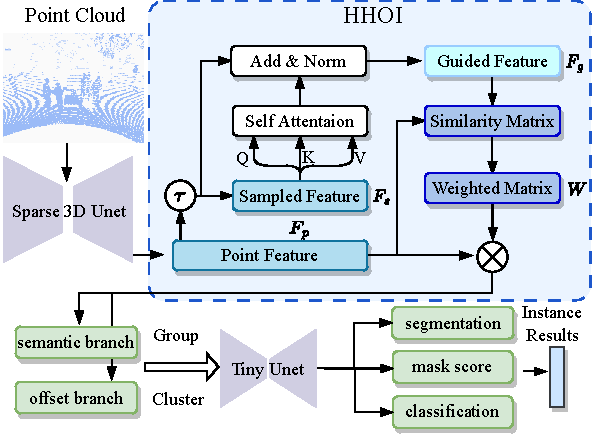
\includegraphics[width=0.98\columnwidth]{pic/seg.pdf}
    \caption{ The architecture of our segmentation method. Especially, the HHOI module extracts the correlation within different persons and the human-object relationships, which can benefit the point-wise and instance-wise classification.
    %The point cloud is fed in Sparse 3D Unet to extract the point feature. Then, the HHOI module extracts the correlation within different persons and the human-object relationships. After that, two branches are constructed to output the point-wise semantic scores and offset vectors and we obtian the final results through a tiny Unet.
    }
    \label{fig:segnetwork}
    \vspace{-3ex}
\end{figure}

\subsubsection{Point-wise Prediction and Refinement}
Taking the weighted features as input, the semantic branch and offset branch apply two-layer MLP and output the semantic scores $S\in \mathcal{R}^{N \times K}$ and offset vectors  $O\in \mathcal{R}^{N \times K}$  from the point to the instance center, respectively. The weighted cross-entropy loss $\mathcal{L}_{\text {semantic}}$ and $L_1$ regression loss $\mathcal{L}_{\text {offset}} $ are used to train the semantic and offset branches. After that, we follow the refinement stage in SoftGroup~\cite{vu2022softgroup}, where point-level proposals are fed into a tiny-unet to predict classification scores, instance masks, and mask scores to generate the final instance results. Specifically, the classification branch predicts the category scores $c_k$ for each instance. The segmentation branch utilizes a point-wise MLP to predict an instance mask $m_k$ for each instance proposal. Mask scoring branch estimates the IoU between the predicted mask and the ground truth for each instance. We train each branch with cross-entropy loss $\mathcal{L}_{\text {class}}$, binary cross-entropy loss $\mathcal{L}_{\text {mask}}$, and $l_2$ regression loss $\mathcal{L}_{\text{mask score}}$. And the total loss is the sum of all above losses.
%$\mathcal{L} = \mathcal{L}_{\text {semantic}}+\mathcal{L}_{\text {offset}}+\mathcal{L}_{\text {class}}+\mathcal{L}_{\text {mask}}+\mathcal{L}_{\text{mask score}}.$
% ------------ move to supp
% $$
% L_{\text {semantic }}=\frac{1}{N} \sum_{i=1}^N \operatorname{CE}\left(\boldsymbol{s}_i, s_i^*\right),$$
% $$
% L_{\text {offset }}=\frac{1}{\sum_{i=1}^N \mathbb{I}_{\left\{\boldsymbol{p}_i\right\}}} \sum_{i=1}^N \mathbb{I}_{\left\{\boldsymbol{p}_i\right\}}\left\|\boldsymbol{o}_i-\boldsymbol{o}_i^*\right\|_1,
% $$
% $$
% L_{\text {class }}=\frac{1}{K} \sum_{k=1}^K \mathrm{CE}\left(\boldsymbol{c}_k, c_k^*\right), 
% $$
% $$
% L_{\text {mask }}=\frac{1}{\sum_{k=1}^K \mathbb{I}_{\left\{\boldsymbol{m}_k\right\}}} \sum_{k=1}^K \mathbb{I}_{\left\{\boldsymbol{m}_k\right\}} \mathrm{BCE}\left(\boldsymbol{m}_k, \boldsymbol{m}_k^*\right), 
% $$
% $$
% \mathcal{L}_{\text{mask score}}=\frac{1}{\sum_{k=1}^{N_{g t}} \mathbb{I}_{\left\{iou_k\right\}}} \sum_{k=1}^{N_{g t}} \mathbb{I}_{\left\{iou_k\right\}}\left\|iou_k-iou_k^*\right\|_2
% $$
% where $*$ denotes the ground truth.





\begin{figure}[t]
    \centering
    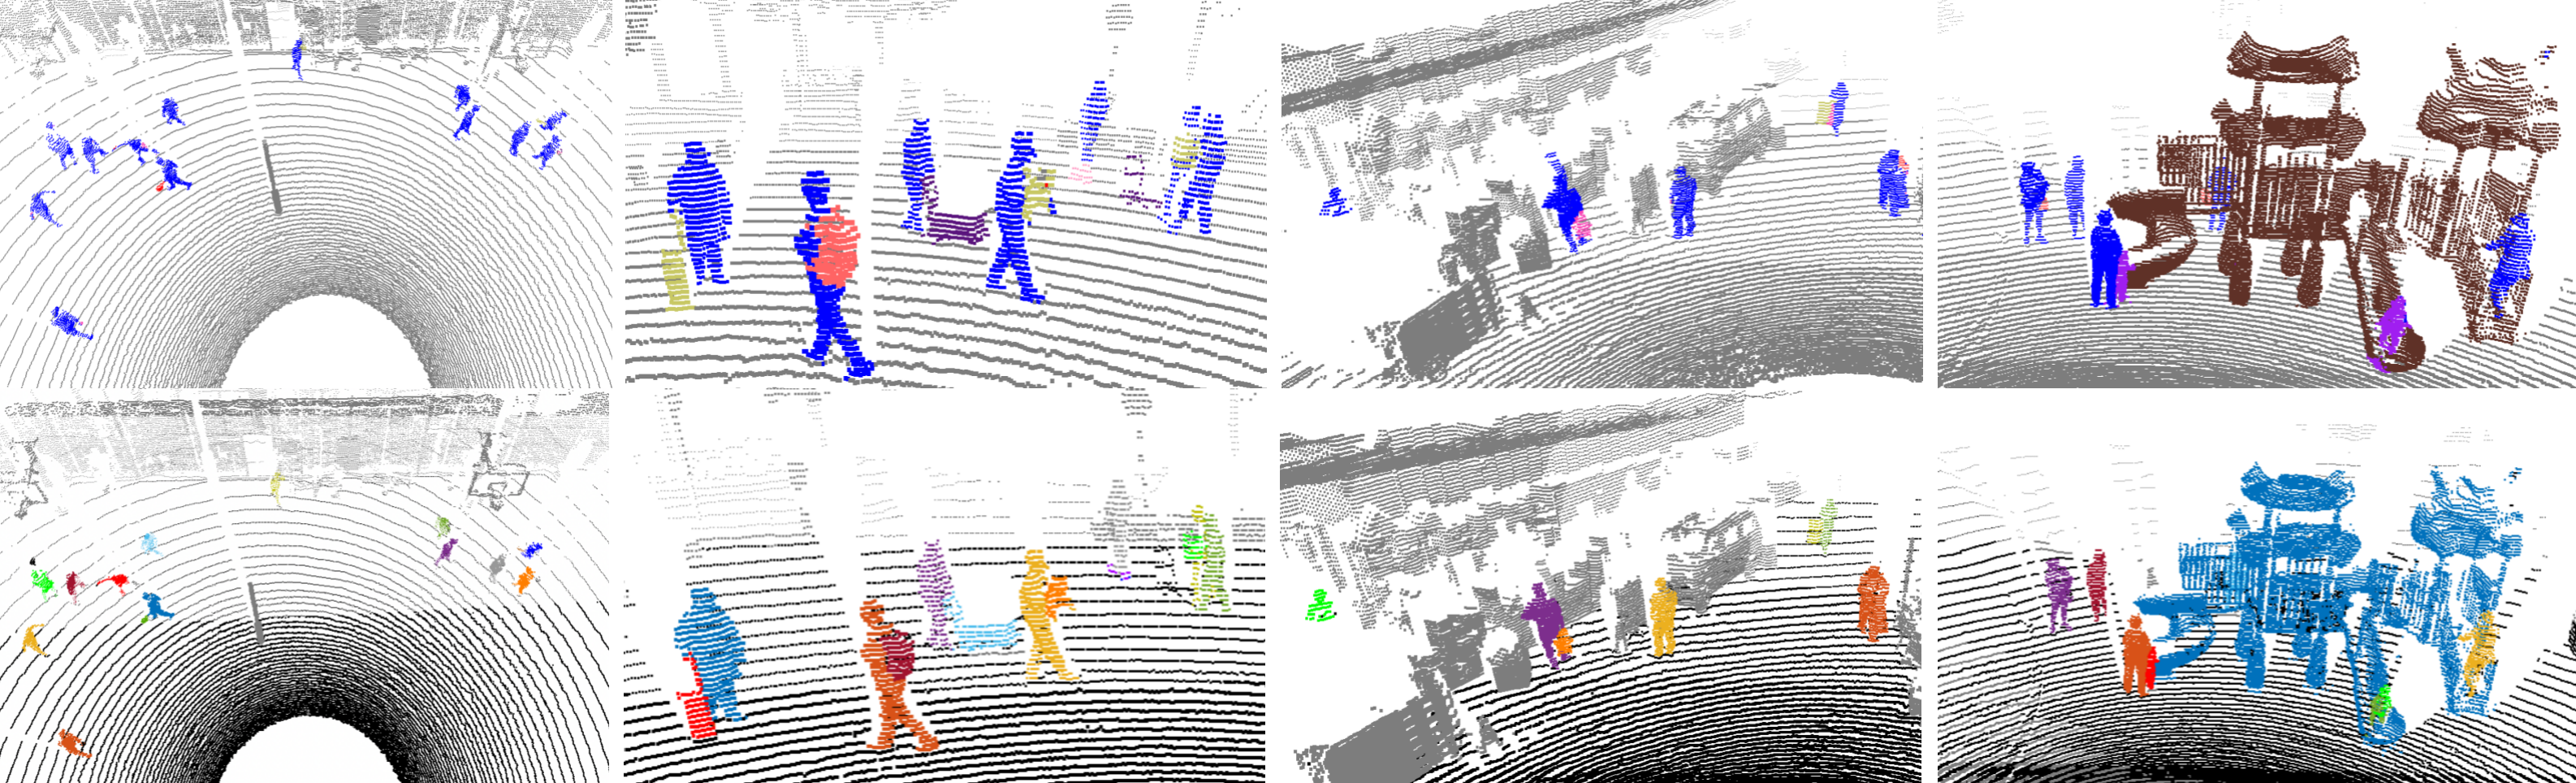
\includegraphics[width=1\columnwidth]{pic/exp-seg.png}
    \caption{The visualization of semantic (first row) and instance (second row) segmentation results of our method on HuCenLife. }
    \label{fig:vis}
   \vspace{-2ex}
\end{figure}



\subsection{Experiments}
\subsubsection{Baselines and Evaluation Metrics}
Previous 3D instance segmentation works can be divided into LiDAR-based methods and RGB-D-based methods. For the former, we compare with current SOTA method DSNet ~\cite{hong2021lidar} of both voxel-division version and cylinder-division version. For the latter, we select current SOTA approaches DKnet ~\cite{wu20223d} and SoftGroup~\cite{vu2022softgroup} for comparison. 


%We present several popular baselines with different modalities for segmentation.
%Previous methods can be divided into LiDAR-based and RGB-D based. We evaluate the result on the LiDAR-based methods Voxel-based DSNet and Cylinder-based DSNet\cite{hong2021lidar}, and the RGB-D based instance segmentation baselines DKnet\cite{wu20223d} and Softgroup\cite{vu2022softgroup}.
%For LiDAR-Camera modality, we apply two fusion strategies (PointPainting and LocalFusion) on our methods. The fusion baselines are provided to facilitate further exploration. PointPainting appends the raw LiDAR point with corresponding RGB color according to calibration matrix. LocalFusion concatenates high-dimensional image feature to the corresponding high dimensional point semantic feature. Our HHOI module has consistently improved the performance on various fusion strategies, validating its generalization ability.
% And we also apply our HHOI on each fusion baseline to validate the generalization ability of our method. 

%\subsubsection{Evaluation Metrics}
We utilize mean IoU (mIoU) to evaluate the quality of the semantic segmentation. For instance segmentation, we report AP50 and AP25 which denote the scores with IoU thresholds of 50\% and 25\%, respectively.

\subsubsection{Results}

\noindent\textbf{Comparison on HuCenLife dataset. } 
We compare the results of our proposed method with baseline methods in Table ~\ref{tab:test}. DSNet does not get satisfactory results, mainly because it focuses on traffic scenarios, while the span of object scale is much larger in human-centric scenarios. SoftGroup is better than outdoor methods because it has a refinement stage for recognizing small objects. Our method performs best due to the use of interaction information.

%With the help of HHOI, the network learns a better human-human interaction representation and the object features are enhance by human-guided feature, and our methods outperforms baselines on contemporary benchmarks.



\noindent\textbf{Comparison on BEHAVE dataset. } 
To further evaluate the generalization capability of human-object interaction scenes, we also conduct experiments for semantic segmentation on BEHAVE~\cite{bhatnagar2022behave} dataset in Table ~\ref{tab:behave}. BEHAVE dataset is a human-object interaction dataset, which is collected in indoor scenarios and provides RGB-D frames and 3D SMPL. To adapt it to our task, we generate the point cloud and segmentation label from RGB-D images and segmented masks. There is only single person with single object per frame and the total number of the object categories is 20. We follow the official protocol of dataset splitting. Our method still outperforms the best baseline method SoftGroup by 2.8\% in mIOU. 
%The results validate the generalizability and the effective ness of our HHOI module.

\noindent\textbf{Sensor-fusion-based 3D segmentation. }
Because our dataset also contains image data, we also provide LiDAR-Camera sensor-fusion baselines based on our method in Table ~\ref{tab:test} to facilitate further research. PointPainting appends the raw LiDAR point with corresponding RGB color according to calibration matrix. LocalFusion concatenates high-dimensional image feature to the corresponding high dimensional point semantic feature. And our HHOI module has consistently improved the performance on various fusion strategies, validating its generalization ability.

%Pointpainting get a comparable result with the LiDAR-only backbone, while LocalFusion perform better with a little margin, which demonstrates the effectiveness to introduce image features in higher dimensions.
%We apply our HHOI on each fusion strategies, our results demonstrate that our module consistently improves the performance on each fusion baseline.


\begin{table}[ht]
  \centering
    \caption{Person-only 3D detection results on HuCenLife. }
    \label{tab:humdetectionresult}
    \setlength{\tabcolsep}{0.8mm}
\begin{tabular}{{l|ccc|l}}
\hline
Methods      & AP(0.25) & AP(0.5) & AP(1.0) & mAP  \\ \hline
CenterPoint\cite{centerpoint}  & 61.8    & 68.7    & 70.3    & 66.9 \\
STCrowd\cite{cong2022stcrowd}      &  61.8    &  71.6   & 73.4   & 68.9 \\
TED\cite{TED}          &  51.0    &  53.3   &  54.1   & 52.8 \\
CenterFormer\cite{centerformer} &   73.0   & 80.1    & 81.4    & 78.2 \\ 
\hline
\end{tabular}
\vspace{-3ex}
\end{table}

\begin{table}[ht]
\caption{Full-category 3D detection results (AP) on HuCenLife. We only select six types of objects for demonstration.}

\label{tab:objectdetection}
\setlength{\tabcolsep}{1.3mm}
\resizebox{\linewidth}{!}{      
\begin{tabular}{l|c|c|c|c|c|c}
\hline
Methods     & motorbike   & box          & cart        & scooter & backpack     & object in hand          \\ \hline
CenterPoint\cite{centerpoint} &13.4  & 17.1          & 20.9             & 43.4 & 4.2          &  8.4             \\ \hline
STCrowd\cite{cong2022stcrowd}     &   5.4        & 14.4 & 25.3  & 48.7          & 4.5 & 13.5 \\ \hline
CenterFormer\cite{centerformer}     & 3.8          & 16.2 & 24.2  & 44.4         & 2.6 & 12.5 \\ \hline
\end{tabular}
}
\vspace{-3ex}
\end{table}
%-------------------------------------------------------------------------
\section{Human-centric 3D Detection}
\label{sec:detect}
\begin{figure*}[t]
    \centering
    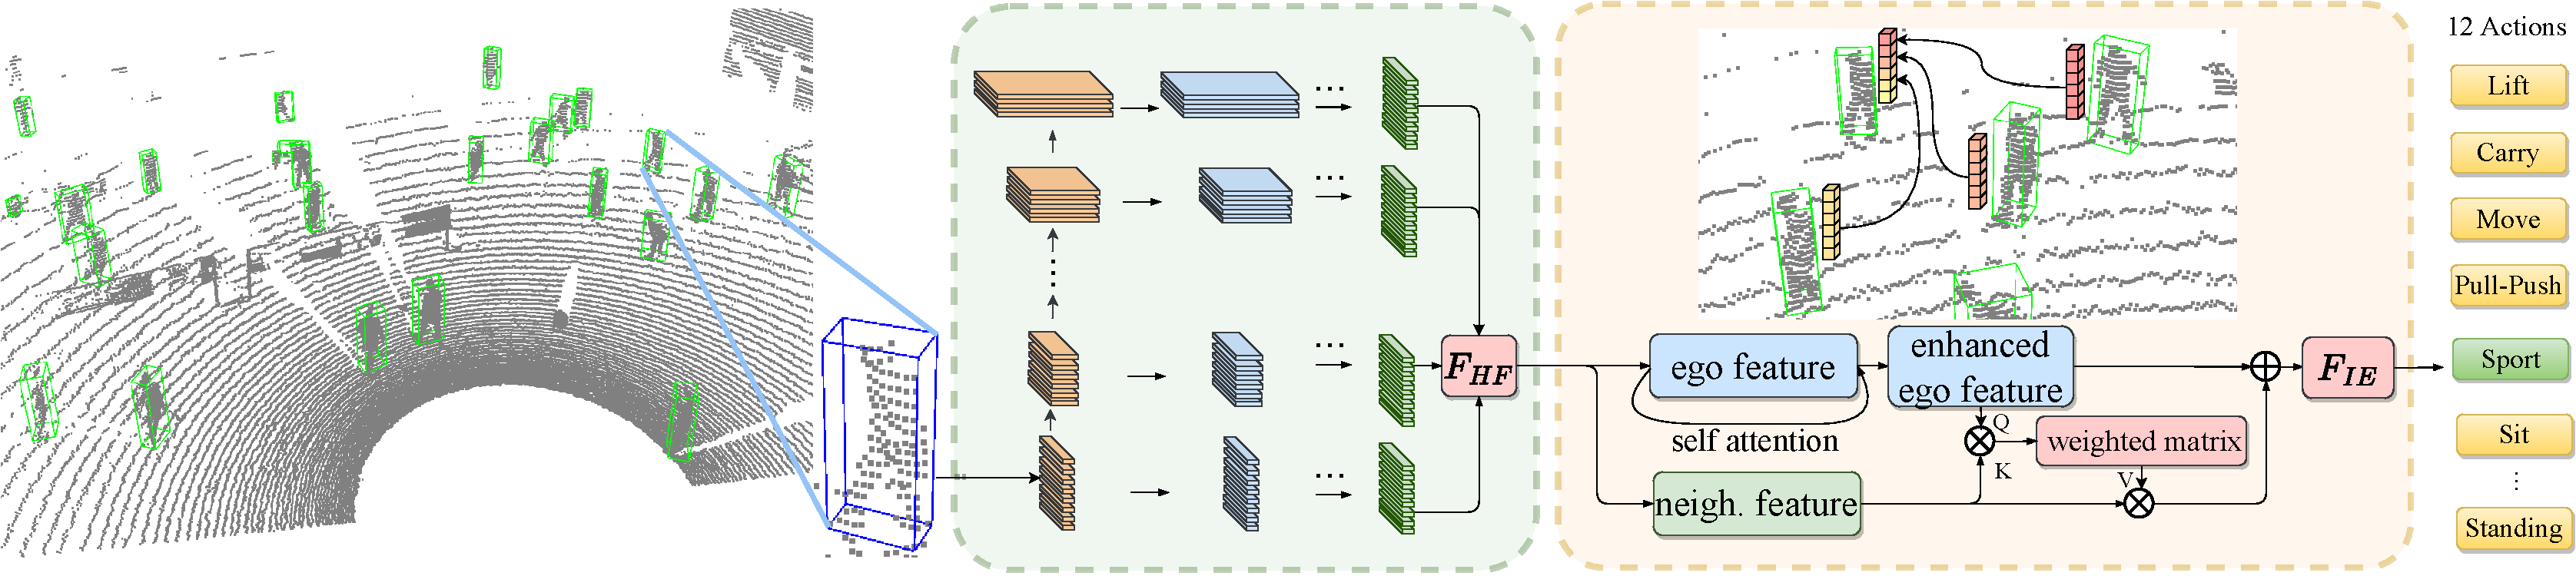
\includegraphics[width=2\columnwidth]{pic/pointMRNet.drawio.pdf}
    \caption{Pipeline of our method for human-centric action recognition. We first utilize 3D detector to obtain a set of bounding boxes of persons. Then, for each person, we extract multi-resolution features and get a hierarchical fusion feature $F_{HF}$. Next, we leverage the relationship with neighbors to enhance the ego-feature and obtain a comprehensive feature $F_{IE}$ for the final action classification.
     %Hierarchical Fusion Feature and $F_{IEE}$ means Interaction Enhanced Ego Feature. The single person's point cloud cropped by bounding box is fed in HPFE to extract multi-scale features. After that, ENFI will explore the interactive relationship between ego feature and neighbour feature.
     }
    \label{fig:MRNetnetwork}
    \vspace{-1ex}
\end{figure*}


LiDAR point cloud-based 3D detection is well-studied in recent years, driven by autonomous driving. It provides critical information of obstacles for the motion planning of robots to guarantee the safety. Specifically, the input for 3D detection is the point cloud $P$ and the output is predicted bounding boxes with 7 dimensions ($x$,$y$,$z$,$w$,$l$,$h$,$r$), consisting of the 3D position in LiDAR coordinate system, the size of bounding box, and the rotation. In this section, we provide benchmarks for the 3D detection task on HuCenLife by evaluating current state-of-the-art methods and give discussion on the research of human-centric 3D detection.


%Detection can benefit many downstreams tasks such as action recognition, tracking, trajectory prediction and etc. Existing datasets are either collected in traffic scenarios or in crowded, and the pedestrians have limited action, like walking and standing. While in real world, human have diverse actions including sitting, playing sports, hugging, doing fitness, etc. Different human poses lead to various of size of human bounding box, making the accurate detection harder.


%When detecting objects, their bounding box size can also vary greatly, even within the same category. Additionally, algorithms need to determine whether an object is being interacted with, which presents a new challenge.(added)

%Specifically, the input of the detection is the point cloud $P$ and the output is bounding box with 7 dimensions ($x$,$y$,$z$,$w$,$l$,$h$,$r$).
%We provide several baselines in following.

 % Human-centric 3D Detection is a task to detect the
% location of all the human in thegiven point cloud. Detection is the foundation of many other tasks such as  action recognition, tracking, trajectory prediction and etc. For existing dataset, they only focus on pedestrian. This narrow them down onto person who is either walking or standing. However it's obvious that a person can't be walking or standing out-door 24 hours a day, he or she will have more actions, such as sitting, playing sports, hugging, doing fitness and so on. Different actions led to different human shapes. Abundant actions in our dataset which contribute to the variousness of human shapes and covering both in-door and out-door help our dataset represents the really world better. We provides baseline on this unique challenge here. 



\subsection{Baselines and Evaluation Metrics}
We choose four representative works and test their performance on our dataset. CenterPoint ~\cite{centerpoint} is a popular anchor-free detector and based on it, STCrowd ~\cite{cong2022stcrowd} aims at solving dense crowd scenarios. By means of the transformer mechanism, TED~\cite{TED} and CenterFormer~\cite{centerformer} achieve impressive performance recently. Following ~\cite{cong2022stcrowd,caesar2020nuscenes}, we use Average Precision (AP) with 3D center distance thresholds D = \{0.25, 0.5, 1\} meters as the evaluation metric. Then mean Average Precision (mAP) is obtained by averaging AP.

 % For current SOTA 3D detection. We choose TED\cite{TED} and Centerformer\cite{centerformer}. 
 %Current 3D detection methods TED\cite{TED} and Centerformer\cite{centerformer} utilize transformer strategies, the former extract transformation-equivariant feature for detection and the latter apply a deformable transformer to aggravate feature from  candidate center.
 %We provide the experiments based on above baselines.

%\subsection{Evaluation Metrics}
 %\textbf{Average Precision metric.}Following \cite{nuScenes，STcrowd}, we use Average Precision (AP) with 3D center distance threshold D = {0.25, 0.5, 1} meters. Then mean Average Precision (mAP) is obtained by averaging AP.
%\begin{equation}
%m A P=\frac{1}{|D|} \sum_{d \in D} A P_d
%\end{equation}

\subsection{Results and Discussion}

We conduct experiments on two settings, including \textbf{person-only 3D detection} in Table ~\ref{tab:humdetectionresult} and  \textbf{full-category 3D detection} in Table ~\ref{tab:objectdetection}. These baseline methods are designed for large-scale traffic scenarios, which perform limited on human-centric scenarios, especially for detecting small objects. We conclude with three main challenges for conducting 3D detection in human-centric scenarios. First, people usually have different poses in different actions, such as crouching, sitting, waving, etc., and such diverse body poses cause distinct sizes of bounding box. Second, there are many relatively small objects in scenes, bringing difficulties to balance the accuracy of fine-grained detection and the efficiency of large-scale scene data processing. Third, multi-objects may locate at different heights in the same place, such as in complex scenarios of escalator and slide, leading to larger dimension of feature recognition. Previous methods using BEV feature map will miss details and transformer-based methods have horrible cost. Therefore, there is a lot of room for the 3D detection research in human-centric scenes, while our dataset can offer a good platform for it.


%However, the 3D Lidar detection algorithms are optimized for road scenes and struggle with interference from common daily-life objects like sculptures, chairs, and express boxes. Ceilings in indoor environments negatively affect their use of the bird's-eye-view feature map. Moreover, detecting individuals on staircases and escalators with significant altitude differences poses a significant challenge.
%For future work, improvement can be achieved though gaining a deeper understanding of whether the instance is human or not, having the ability to suit both indoor and out-door and handle large scene and small scene.


%We compare the results of baselines in Table \ref{tab:humdetectionresult}. Compared to others\cite{centerformer,STcrowd,centerpoint}, TED\cite{TED} is the only anchor-based detection algorithm which limits its performance. Unlike cars focused by auto-mobile dataset\cite{nuScenes,Geiger2013VisionMR}, human can have really different bounding box shape. This narrows down the performance of anchor-based algorithm. Despite STcrowd\cite{STcrowd} utilizes multi-scale feature for dense crowd detection, this design make it more vulnerable towards interference created by the object being interacting with. Centerformer\cite{centerformer} and Centerpoint\cite{centerpoint} have achieved reasonable performance, with centerformer being slightly higher attribute to its transformer design. 


%However, none of the algorithm have been optimized for other than road scene. So they wasn't design to withstand the interference created by items look like sheltered human In daily-life scenarios, such as sculpture, chair， big express box, etc. Also, ceiling in the indoors will have negative effect on the bev feature map which is popularly used by current detection algorithms\cite{TED,centerformer,STcrowd,centerpoint}. Furthermore, different from the existing dataset, we have huge altitude difference between person in the scene caused by stairs and escalator. This is challenging for current algorithm to detect person accurately on these facilitates.
% However, The current algorithms\cite{TED,centerformer,STcrowd,centerpoint} for 3D Lidar detection have been optimized primarily for road scenes and is not able to withstand the interference created by objects that are commonly found in daily-life scenarios, such as sculptures, chairs, and large express boxes. Additionally, the presence of ceilings in indoor environments can have a negative effect on the bird's-eye-view (BEV) feature map used by them. Another significant challenge for them is the presence of significant altitude differences between individuals in a scene, particularly when staircases and escalators present.




%\subsubsection{Full-category 3D Detection}
%Specifically, to accomplish the task, two separate models are trained, one for detection human and one for object. We show AP result of part of the classes in Table \ref{tab:objectdetection}. Results show that the disadvantage of current 3d detection have been further magnified. For future work, it need to have a understanding of the relation between object and person. Additionally, better NMS algorithms are needed to address the issue of object bounding box collides with human bounding box.
%However, this has revealed that while CenterPoint remains a popular choice for 3D object detection, it is not well-suited for our unique dataset due to the inherent challenges it poses. Unlike outdoor datasets that focus on objects such as cars, trucks, and humans, whose sizes are typically similar and distinct from one another, our dataset specifically targets human-object interactions, such as individuals carrying bags or using computers, where the bounding boxes of the objects may intersect or be in close proximity to one another. This poses a challenge for conventional outdoor detection methods, including those based on bev heatmap and non-maximum suppression (NMS) designs, such as CenterPoint, and limits their performance.Furthermore, Our outdoor scenes exhibit a level of sparsity that current indoor methods are ill-equipped to handle, as they are typically designed for smaller indoor datasets. This mismatch in scale and complexity poses a significant challenge for the application of existing indoor methods to our unique outdoor context.

% For future algorithms, it's required to have an enhanced understanding of the relationship between humans and objects. Being able to whether objects that are being interacted or not even in close distance to human. The size of objects human interacts with can vary dramatically, thus algorithms should have a better dynamic receptive field to accommodate these varying object sizes. Finally, to address the issue of object instance collision, better NMS algorithms are required. Conventional NMS designs are not suitable for this tasks, where objects may intersect or be in close proximity to one another. Therefore, developing algorithms that can effectively handle object collision is necessary.





%-------------------------------------------------------------------------

\section{Human-centric Action Recognition}
\label{sec:action}

Previous works for action recognition are based on 2D images or videos and they only need to give one label for one scene. We introduce the 3D action recognition task in large-scale human-centric scenarios, which aims to detect all persons in the scene and provide corresponding action types. 3D action recognition task is significant for fine-grained scene understanding and can benefit the development of intelligent surveillance and collaborative robots. To our knowledge, we are the first to propose the related dataset and solutions for the new task. 


%The input of human-centric action recognition is a frame of point cloud $P$ and we propose an end-to-end two-stage model HuCenAction that first detects the human location and then predicts the action category. 
%Human behavior is complex and closely related to the surrounding objects and other people. For one perspective, the size of the objects that interacting with people is various, thus we leverage multi-resolution Hierarchical Point Feature Extraction(HPFE) to capture global features and local features. In addition, considering the interaction between the human and the surrounding neighbours, we design Ego-Neighbour Feature Interaction(ENFI) to get the enhanced human feature and benefit the action classification.
\subsection{Method}
Our 3D action recognition method is in a two-stage manner based on the input of LiDAR point cloud, as shown in Figure ~\ref{fig:MRNetnetwork}. Considering that some human actions are related to adjacent interactive objects, after obtaining individual bounding box by 3D detector, we enlarge the box to crop more points related to the person for the following fine-grained feature extraction. Especially, we leverage a Hierarchical Point Feature Extraction module to pay attention to multi-scale objects and get multi-level features. Moreover, we design an Ego-Neighbour Feature Interaction (ENFI) module to make use of the relationship among the ego-person and neighbors to help forecast social actions. 

\subsubsection{Hierarchical Point Feature Extraction}
%For daily-life scenarios, the objects interacted with people have varying sizes. However, most point cloud classification methods lack the ability to capture local features with diverse receptive fields. 

To capture both global features and local features with dynamically changing receptive fields, we use $R$ parallel branches to extract multi-resolution features.
Serial Set Abstractions~\cite{qi2017pointnet} are applied to process the features of different scales, where each branch undergoes $L$ times with fixed sampling cores and branch-specific sampling range. Finally, these features are up-sampled to the same dimension and fused together with pooling to generate the hierarchical fusion feature $F_{HF}$.

%To capture both global features and local features with dynamically changing receptive fields, we designed HPFE, which has $R$ parallel resolution branches to hierarchically extract features from $R$ resolutions $F_i \in \mathcal{R}^{(N/2^r) \times (32*2^r)}$. 
%Serial Set Abstractions(SA)~\cite{qi2017pointnet} is applied to process the features of different scales, where each branch undergoes L times with fixed sampling core and branch-specific sampling range to extract increasingly specific features.
% Serial Set Abstractions(SA) are applied to each branch to perceive the features of a specific scale $L$ times with fixed sampling core and branch-specific sampling range. 
%$$F_i^{l+1} = SA(F_i^l), \quad i=0,1,...,R,l=0,1,...,L$$
 %Finally, these features are up-sampled to the same dimension and fused and pooled to generate Hierarchical Fusion Features $F_{HF} = \text{Pool}({\text{UpSample}(F_i^l)})$.
 
% Finally, the features of R branches will be up-sampled to same dimension, and then we fuse and pool the features of different resolutions to generate Hierarchical Fusion Feature $F_{HF} = \text{Pool}({F_i})$.
 % HPFE incorporates a Scalable Equal Sampling stage to fully perceive the features of a specific scale for each resolution channel and increase the learning ability of the network.
% For each point of single person, we use Set Abstraction for $R$ resolution branches: $P_i \in R^{(N/2^r) \times (32*2^r)}$.
% Then, the features of these channels are simultaneously input into the Scalable Equal Sampling Module for equal sampling. 
% The sampling core remains unchanged during this process, but the receptive field gradually expands with the increase of network depth. 
% And the depth of the network can be a?
\subsubsection{Ego-Neighbour Feature Interaction}

%Human behavior is also related the behavior of people around him. So we design Ego-Neighbour Feature Interaction(ENFI) to perceive the interaction with neighbors.
Like Figure ~\ref{fig:MRNetnetwork} shows, we first enhance the ego person feature by self-attention and get $F_{ego}$. Then, we select features of $k$ neighbours around the target as $K_{neigh}$ and $V_{neigh}$ and take the ego-feature as queries $Q_{ego}$. The distances from neighbours to the target are used for position encoding. 
%First, the feature of a ego person is enhanced by self-attention, and then the enhanced ego feature $F_{ego}$ will be used as $Q_{ego}$ for following cross attention with neighbours. 
%We select k neighbours feature around the target as $K_{neigh}$ and $V_{neigh}$.
%The distances from neighbours to ego are for position encoding.
We apply cross-attention to extract the ego-neighbour interaction information and gain the final interaction enhanced ego feature by $F_{IE} = F_{ego} \bigoplus \text{CrossAttention}(Q_{ego},K_{neigh},V_{neigh})$, where $\bigoplus$ denotes concatenation. In this way, we model the relationships of a group to benefit the social action recognition.

%Thus we take full advantage of human-human interaction to benefit the instance action recognition.

%First, the feature of a ego person is enhanced by self-attention, and then the enhanced ego feature $F_{ego}$ will be used as $Q_{ego}$ for following cross attention with neighbours. 
%We select k neighbours feature around the target as $K_{neigh}$ and $V_{neigh}$. The distances from neighbours to ego are for position encoding. Then we apply cross-attention to extract the ego-neighbour interaction and concatenate with enhanced ego feature to get final Interaction Enhanced Ego Feature $F_{IEE} = F_{ego} + \text{crossattention}(Q_{ego},K_{neigh},V_{neigh})$. 
%Thus we take full advantage of human-human interaction to benefit the instance action recognition.
% We get the features of $k+1$ neighbours where k is the number of selected neighbour. 
% We use the distance from ego as position encoding. After self attention, we get the enhanced ego feature which will be used as $Q$ for following cross attention. The features of k neighbors will be used as $K$ and $V$ after linear projection. 
% $K_{neigh}$ will be multiplied by $Q_{Ego}$, and then scale and normalize to get attention affinity matrix, which means the attention coefficient of ego feature for other neighbor.
% $$M_{aff}=softmax(Q_{ego} \cdot K_{nei} / \sqrt{d})$$
% Then, the attention affinity matrix is finally multiplied by $V_{neigh}$ to obtain the weighted features of neighbor of interest to ego.
% $$F_{weighted}=M_{aff} \cdot V_{nei}$$


\iffalse

\begin{table*}[ht]
  \centering
    \caption{Human-centric Action Recognition Result}
    \label{tab:endtoend}
    \setlength{\tabcolsep}{1mm}
    
\resizebox{\linewidth}{!}{      

\begin{tabular}{l|cccccccccccc|ccc}
\hline
Methods            & Lift & Carry & Move & Pull-Push & Sit  & Scooter-BalanceBike & Hum-Inter & Fitness & Entertain & Sports & Bend-Over & Standing & mAP  & mRec & mPrec \\ \hline
Centerpoint\cite{centerpoint}        & 0.3  & 2.7   & 0.1  & 8.6       & 2.2  & 18.1                & 0.0       & 0.0     & 0.6       & 4.7    & 0.1       & 18.7     & 4.7  & 16.3 & 17.8  \\
STCrowd\cite{STcrowd}            & 0.2  & 0.8   & 0.1  & 15.6      & 3.3  & 14.5                & 0.0       & 4.3     & 0.4       & 3.0    & 0.4       & 23.0     & 5.5  & 16.7 & 21.0  \\
CenterFormer\cite{centerformer}       & 0.9  & 0.0   & 0.0  & 0.0       & 6.4  & 0.0                 & 0.0       & 0.0     & 2.0       & 58.7   & 0.0       & 13.7     & 6.8  & 20.3 & 11.4  \\ \hline
Centerpoint-HCA  & 2.7  & 11.3  & 9.1  & 19.4      & 16.3 & 46.2                & 2.2       & 1.4     & 4.4       & 22.6   & 2.4       & 9.7      & \textbf{12.3} & \textbf{40.0} & \textbf{26.9}  \\
STCrowd-HCA      & 2.1  & 10.1  & 8.1  & 16.4      & 14.1 & 44.2                & 1.9       & 2.4     & 3.9       & 17.9   & 1.8       & 8.8      & 11.0 & 37.5 & 25.8  \\
CenterFormer-HCA & 2.7  & 8.3   & 7.0  & 18.1      & 13.4 & 52.7                & 1.7       & 1.8     & 3.8       & 21.4   & 2.0       & 8.1      & 11.7 & 37.6 & 26.8  \\ \hline
\end{tabular}

}
\vspace{-1ex}
\end{table*}


\begin{table}[ht]
\caption{Ablation Study on Classification Network,* means multi-scale grouping PointNet++. We show mean Average Precision(mAP), mean Recall(mRec), and mean Precise(mPrec).}
\label{tab:secondstage}
\begin{tabular}{l|ccc}

\hline
\multicolumn{1}{l|}{Methods} & mAP  & mRec & mPrec \\ \hline
ViT\cite{dosovitskiy2020image}                          & 6.8  & 23.1 & 19.9  \\ \hline
PVT\cite{zhang2022pvt}                          & 6.8  & 30.5 & 19.8  \\
PointNet\cite{qi2017pointnet}                     & 4.6  & 26.3 & 15.5  \\
PointNet++\cite{qi2017pointnet++}              & 8.2  & 34.2 & 22.7  \\
PointNet++*           & 7.4  & 34.6 & 20.6  \\
PointMLP\cite{ma2022rethinking}                     & 6.1  & 28.0 & 19.4  \\
PointNeXt\cite{qian2022pointnext}                    & 8.0  & 33.0 & 21.2  \\ \hline
HCA(w/o ENFI)         & 9.3  & 37.1 & 24.7  \\
HCA                  & 12.3 & 40.0 & 26.9  \\ \hline
\end{tabular}
\end{table}

\fi



\begin{table}[ht]
\caption{Comparison results of action recognition on HuCenLife. All methods are based on the same 3D detector for fair evaluation.}
\label{tab:actioncompare}
\begin{tabular}{l|ccc}

\hline
\multicolumn{1}{l|}{Methods} & mAP  & mRecall & mPrecision \\ \hline
Baseline & 7.3  & 14.6 & 19.9\\\hline
+ ViT\cite{dosovitskiy2020image}                          & 9.4  & 23.1 & 19.9  \\ \hline

+ PVT\cite{zhang2022pvt}                          & 13.2  & 30.5 & 19.8  \\
+ PointNet\cite{qi2017pointnet}                     & 8.4  & 26.3 & 15.5  \\
+ PointNet++\cite{qi2017pointnet++}              & 15.6  & 34.2 & 22.7  \\
+ PointMLP\cite{ma2022rethinking}                     & 11.3  & 28.0 & 19.4  \\
+ PointNeXt\cite{qian2022pointnext}                    & 15.0  & 33.0 & 21.2  \\ \hline

Ours                  & \textbf{21.0} & \textbf{40.0} & \textbf{26.9}  \\ 
Ours(w/o ENFI)         & 15.4  & 37.1 & 24.7  \\
\hline

\end{tabular}
\vspace{-3ex}
\end{table}



\subsection{Experiments}


\subsubsection{Baselines and Evaluation Metrics}
We take pre-trained CenterPoint as the 3D Detector for all the experiments for fair comparison in this section. Because no existing methods can be directly used for solving the new 3D action recognition task. As Table ~\ref{tab:actioncompare} shows, we provide benchmarks and comparisons from four aspects. The first is to directly adapt the 3D detector to predict multi-class persons with different action labels, which is the ``Baseline'' in Table~\ref{tab:actioncompare}. The second is to add a feature extractor for cropped individual point cloud for the second-stage action classification, and we tried several popular point-feature extractors, including PVT, PointNet, PointNet++, PointMLP, and PointNext. In particular, to verify the performance of input modalities, we also use ViT to extract image features for image-based action recognition by projecting the 3D bounding box to calibrated images. At last, we provide the results of our solution with ablation for ENFI module. 

%to crop the single point cloud for it performs best in human detection , and present several point-based classification networks: PointNet, PointNet++, PointMLP and PointNext. We also explore Voxel-based methods such as Point Voxel Transformer.

%There are some ablation studies on modalities comparation. We use 2D bounding box projected from 3D bounding box to get single person's image as the input of Vision Transformer. In addition, we explore the performance gain of ENFI for action recognition.
%\subsubsection{Evaluation Metrics}
% Human-centric Action Recognition is a point cloud classification task. We divide the actions of all people in the data set into 17 categories, and predict an action tag for each person.


 %\textbf{Average Precision metric}. 
 %Following \cite{nuScenes} and \cite{STcrowd}, we use Average Precision (AP) with 3D center distance threshold $D =  \{0.25, 0.5, 1\}$ meters for each action class $C$. 
We use the mean Average Precision (mAP) obtained by averaging AP through thresholds $D =  \{0.25, 0.5, 1\}$ and classes to evaluate the performance.
$$
\mathrm{mAP}=\frac{1}{|\mathbb{C}||\mathbb{D}|} \sum_{c \in \mathbb{C}} \sum_{d \in \mathbb{D}} \mathrm{AP}_{c, d}
$$
where $|\mathbb{C}|$ is the number of action category.
In addition, we also utilize Mean Recall (mRecall) and Mean Precision (mPrecision) by averaging recall and precision through thresholds and classes.

\subsubsection{Results and Discussion}
We show the overall performance in Table ~\ref{tab:actioncompare}, and detailed evaluation values of all categories of actions and visualization results are in the supplementary material. It can be seen from the results that our method outperforms others with an obvious margin, mainly due to the multi-level feature extraction and multi-person interaction modeling, which are more suitable for understanding human-centric complex scenarios. However, our method has its own limitations and there are several potential improvement directions. First, current two-stage framework strongly relies on the detector performance and the one-stage method for action recognition in large-scale scenes is worth exploring. Moreover, human action is time-dependent and how to extract valuable temporal information in consecutive data to eliminate the ambiguity of actions is also promising.  



%\begin{figure*}[t]
%    \centering
%    \includegraphics[width=2\columnwidth]{pic/action_recognition_visulization.png}\caption{Action Recognition visulization. The left figure shows the 3D human bounding box and corresponding actions predicted by our method. The right figure is the ground truth.}
%    \label{fig:vis}
%\end{figure*}
%We compare the impact of Human Detector in Table \ref{tab:endtoend}. Different action involve different amount of movement. Thus, multi-scale feature boost the performance of \cite{centerformer,STcrowd}. Similarly, Centerformer\cite{centerformer} achieve better performance due to the usage of deformable transformer to aggravate feature from and around proposals. However, we observe that single-stage methods can't recognize actions that involved small or large objects and performed poorly in actions that involved objects that shared a similar size to humans. We found that using a refine network improved the performance of the algorithms in these scenarios.

%In addition, we did ablation study on classification network in Table \ref{tab:secondstage}. PointNet++ with multi-scale grouping performs best among all baselines, for it also considers the perception for multi scale features. With the help of HPFE and ENFI, our method captures the features of multiple scales simultaneously and considers the impact of surrounding neighbour, thus finally surpasses PointNet++(msg) 4.9\% in mAP.

%Image-based method does not perform well in crowded scenarios, for the 2D bounding box often include irrelevant people in the backround. And the performance gain of ENFI is 3.0\% in mAP.

















% \begin{equation}
% \mathrm{mRec}=\frac{1}{|\mathbb{C}||\mathbb{D}|} \sum_{c \in \mathbb{C}} \sum_{d \in \mathbb{D}} \mathrm{Recall}_{c, d}
% \end{equation}
% \begin{equation}
% \mathrm{mPrec}=\frac{1}{|\mathbb{C}||\mathbb{D}|} \sum_{c \in \mathbb{C}} \sum_{d \in \mathbb{D}} \mathrm{Precision}_{c, d}
% \end{equation}
% \subsubsection{Implementation Details}

% \subsubsection{Evaluation matrix}


% \end{equation}

% \subsubsection{Result}
% Our result is shown in Table \ref{tab:HuCenAction}


% 3D Human detection evaluation matrix:
% Average Precision (AP) metric with the 3D center distance threshold. For crowded scenes, the distance thresholds are chosen from D = {0.25, 0.5, 1} meters and the mean Average Precision (mAP) is calculated by: (From stcrowd)
% \begin{equation}
% m A P=\frac{1}{|D|} \sum_{d \in D} A P_d
% \end{equation}










%-------------------------------------------------------------------------

\section{More Tasks on HuCenLife}
\label{sec:moretask}
\input{sec/moreTasks}
%-------------------------------------------------------------------------

\section{Conclusion}
\label{sec:conclusion}
\input{sec/conclu}
%-------------------------------------------------------------------------
%\section{Acknowledgements}
%This work was supported by NSFC (No.62206173), Natural Science Foundation of Shanghai (No.22dz1201900), MoE Key Laboratory of Intelligent Perception and Human-Machine Collaboration (ShanghaiTech University), Shanghai Frontiers Science Center of Human-centered Artificial Intelligence (ShangHAI), Shanghai Engineering Research Center of Intelligent Vision and Imaging.
{\small
\bibliographystyle{ieee_fullname}
\bibliography{egbib}
}

%%%%%%%%% APPENDIX
\appendix
\label{sec:appendix}
\clearpage
% \documentclass[10pt,twocolumn,letterpaper]{article}

% \usepackage{iccv}
% \usepackage{times}
% \usepackage{epsfig}
% \usepackage{graphicx}
% \usepackage{amsmath}
% \usepackage{amssymb}


% \usepackage{color}
% \usepackage{times}
% \usepackage{overpic}
% \usepackage{bm}
% \usepackage{tabu}
% \usepackage{bbding}
% \usepackage{multicol}
% \usepackage{multirow}
% \usepackage[table]{xcolor}

% % Include other packages here, before hyperref.

% % If you comment hyperref and then uncomment it, you should delete
% % egpaper.aux before re-running latex.  (Or just hit 'q' on the first latex
% % run, let it finish, and you should be clear).
% \usepackage[pagebackref=true,breaklinks=true,letterpaper=true,colorlinks,bookmarks=false]{hyperref}

% % \iccvfinalcopy % *** Uncomment this line for the final submission

% \def\iccvPaperID{3694} % *** Enter the ICCV Paper ID here
% \def\httilde{\mbox{\tt\raisebox{-.5ex}{\symbol{126}}}}

% % Pages are numbered in submission mode, and unnumbered in camera-ready
% \ificcvfinal\pagestyle{empty}\fi

\begin{appendix}

% %%%%%%%%% TITLE
% \title{Supplement of Human-centric Scene Understanding for 3D Large-scale Scenarios}

% \author{First Author\\
% Institution1\\
% Institution1 address\\
% {\tt\small firstauthor@i1.org}
% % For a paper whose authors are all at the same institution,
% % omit the following lines up until the closing ``}''.
% % Additional authors and addresses can be added with ``\and'',
% % just like the second author.
% % To save space, use either the email address or home page, not both
% \and
% Second Author\\
% Institution2\\
% First line of institution2 address\\
% {\tt\small secondauthor@i2.org}
% }


% \maketitle
% % Remove page # from the first page of camera-ready.
% \ificcvfinal\thispagestyle{empty}\fi


%%%%%%%%% ABSTRACT
\section{Implement details}


\subsection{Human-centric Instance Segmentation}
In HHOI module, the threshold  $\tau$ for sampling high confidence features is set to 0.8 and the number of sampled points $M=256$.
In Point-wise Prediction and Refinement process,
the loss can be formulated as following: 
$\mathcal{L} = \mathcal{L}_{\text {semantic}}+\mathcal{L}_{\text {offset}}+\mathcal{L}_{\text {class}}+\mathcal{L}_{\text {mask}}+\mathcal{L}_{\text{mask score}}.$
$$
L_{\text {semantic }}=\frac{1}{N} \sum_{i=1}^N \operatorname{CE}\left(\boldsymbol{s}_i, s_i^*\right),$$
$$
L_{\text {offset }}=\frac{1}{\sum_{i=1}^N \mathbb{I}_{\left\{\boldsymbol{p}_i\right\}}} \sum_{i=1}^N \mathbb{I}_{\left\{\boldsymbol{p}_i\right\}}\left\|\boldsymbol{o}_i-\boldsymbol{o}_i^*\right\|_1,
$$
$$
L_{\text {class }}=\frac{1}{K} \sum_{k=1}^K \mathrm{CE}\left(\boldsymbol{c}_k, c_k^*\right), 
$$
$$
L_{\text {mask }}=\frac{1}{\sum_{k=1}^K \mathbb{I}_{\left\{\boldsymbol{m}_k\right\}}} \sum_{k=1}^K \mathbb{I}_{\left\{\boldsymbol{m}_k\right\}} \mathrm{BCE}\left(\boldsymbol{m}_k, \boldsymbol{m}_k^*\right), 
$$
$$
\mathcal{L}_{\text{mask score}}=\frac{1}{\sum_{k=1}^{N_{g t}} \mathbb{I}_{\left\{iou_k\right\}}} \sum_{k=1}^{N_{g t}} \mathbb{I}_{\left\{iou_k\right\}}\left\|iou_k-iou_k^*\right\|_2
$$
where $*$ denotes the ground truth.



\subsection{Human-centric Action Recognition}
% \begin{figure*}[t]
%    \centering
%    \includegraphics[width=2\columnwidth]{pic/action_recognition_visulization.png}\caption{Action Recognition visulization. The left figure shows the 3D human bounding box and corresponding actions predicted by our method. The right figure is the ground truth.}
%    \label{fig:vis}
% \end{figure*}
The input for action recognition is frames of large scene point cloud $P\in R^{N\times 4}$ with the 3D location and reflection intensity (x, y, z, r). We extend the length and width of bounding box obtained from human detector by $\Delta h$ and $\Delta w$ respectively, where $\Delta h$ and $\Delta w$ are both set to 0.2 meters. After cropping point clouds with bounding boxes, we use clustering algorithm to find k(k=3) nearest neighbors of the ego point cloud with their relative distances. Next, the point cloud of every single person will be normalized, and sampled by farthest point sample algorithm to n points(n=512). The features of k neighbours and ego will be extracted by HPFE simultaneously to get features of dimension $(k+1) \times c$, which will be input to ENFI afterwards.

In HPFE, we use set abstractions(SA) to down-sample R times on origin point clouds to fork R branches with different resolutions. R is set to 5 by default.
$$P_i \in R^{(n/2^r) \times (32*2^r)} r\in [1,...,R],i\in [1,...,L]$$
where $P_i$ is the feature dimension of R branches. Then we use different sampling radius for the R resolution branches, which are $0.05*(r+1),r\in [1,...,R]$, so that the receptive field of SA will expand with the improving of resolution. After that, we apply equal sampling for L times(L is set to 2) for all branches simultaneously. Finally, we down sample the features of the low-resolution channels to get five features of the same size, which will be fused together to get hierarchical fusion feature.



\section{Dataset details}
\begin{figure}[t]
    \centering
    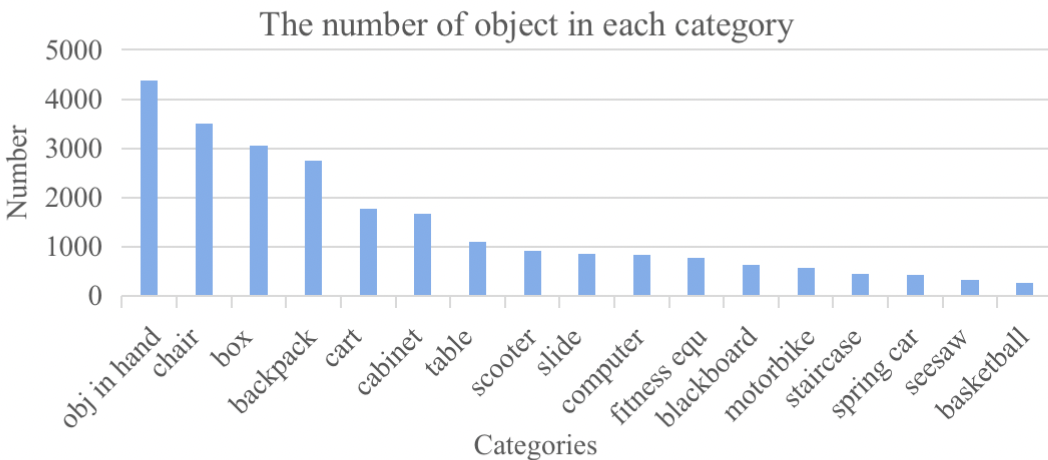
\includegraphics[width=1\columnwidth]{sup-pic/segcount.png}
    \caption{The number of the object for each object.}
    \label{fig:segcount}
    \vspace{-2ex}
\end{figure}


\subsection{Object category for segmentation and detection}
We merge several categories which have low frequency of occurrence and similar geometry shapes in our dataset into a new class, and we also drop some category which only appear in training or testing set with low frequency. The merging list is shown in Table ~\ref{tab:merge}. The categories of objects after merging is 17 and the number of objects in each category is illustrated in Figure. \ref{fig:segcount}.
% Please add the following required packages to your document preamble:
% \usepackage{multirow}

\begin{table}[ht]
\centering
\caption{Object merging list. We merge the categories on the left into the category on the right.}
    \label{tab:merge}
    \setlength{\tabcolsep}{0.8mm}
\begin{tabular}{c|c}
\hline
banner,plank,paper,door,dog,megaphone,guitar  & \multicolumn{1}{c}{\multirow{2}{*}{other}}       \\
toy car,merry go round,car,tricycle,umbrella, & \multicolumn{1}{c}{}                             \\\hline
printer,podium                                &
cabinet                                          \\\hline
bicycle                                       & motorbike                                        \\\hline
{(}two-wheeled{)} {(} self-{)}balancing car   & scooter                                          \\\hline
flat car,stroller,perambulator &cart                                        \\\hline
rockery                                       & slide                                            \\\hline
stool                                         & chair                                            \\\hline
suitcase                                      & box                                              \\\hline
eraser,phone,cup,food,cellphone,red flag,     & \multicolumn{1}{c}{\multirow{4}{*}{obj in hand}} \\
cap,camera,sponge,projector,balloon,          & \multicolumn{1}{c}{}                             \\
plush toy,toy wings,clothes,flower,           & \multicolumn{1}{c}{}                             \\
badminton rocket,handbag,plastic bag,         &
\\\hline\multicolumn{1}{c}{}                            
\end{tabular}
\end{table}


\subsection{Action category for  recognition and detection}
 It is common for a person to perform multiple actions simultaneously. To prioritize these actions, we assign each action to a numerical priority value. We then merge these prioritized actions into 12 categories based on their similarity and frequency of occurrence. Actions with low frequency are dropped to ensure a manageable number of categories. To illustrate this process, we provide a merging Table ~\ref{tab:action_merge} that maps each prioritized action to its corresponding category. The number of each action after the merging process is shown in Figure.~\ref{fig:action_count}.



\begin{figure}[t]
    \centering
    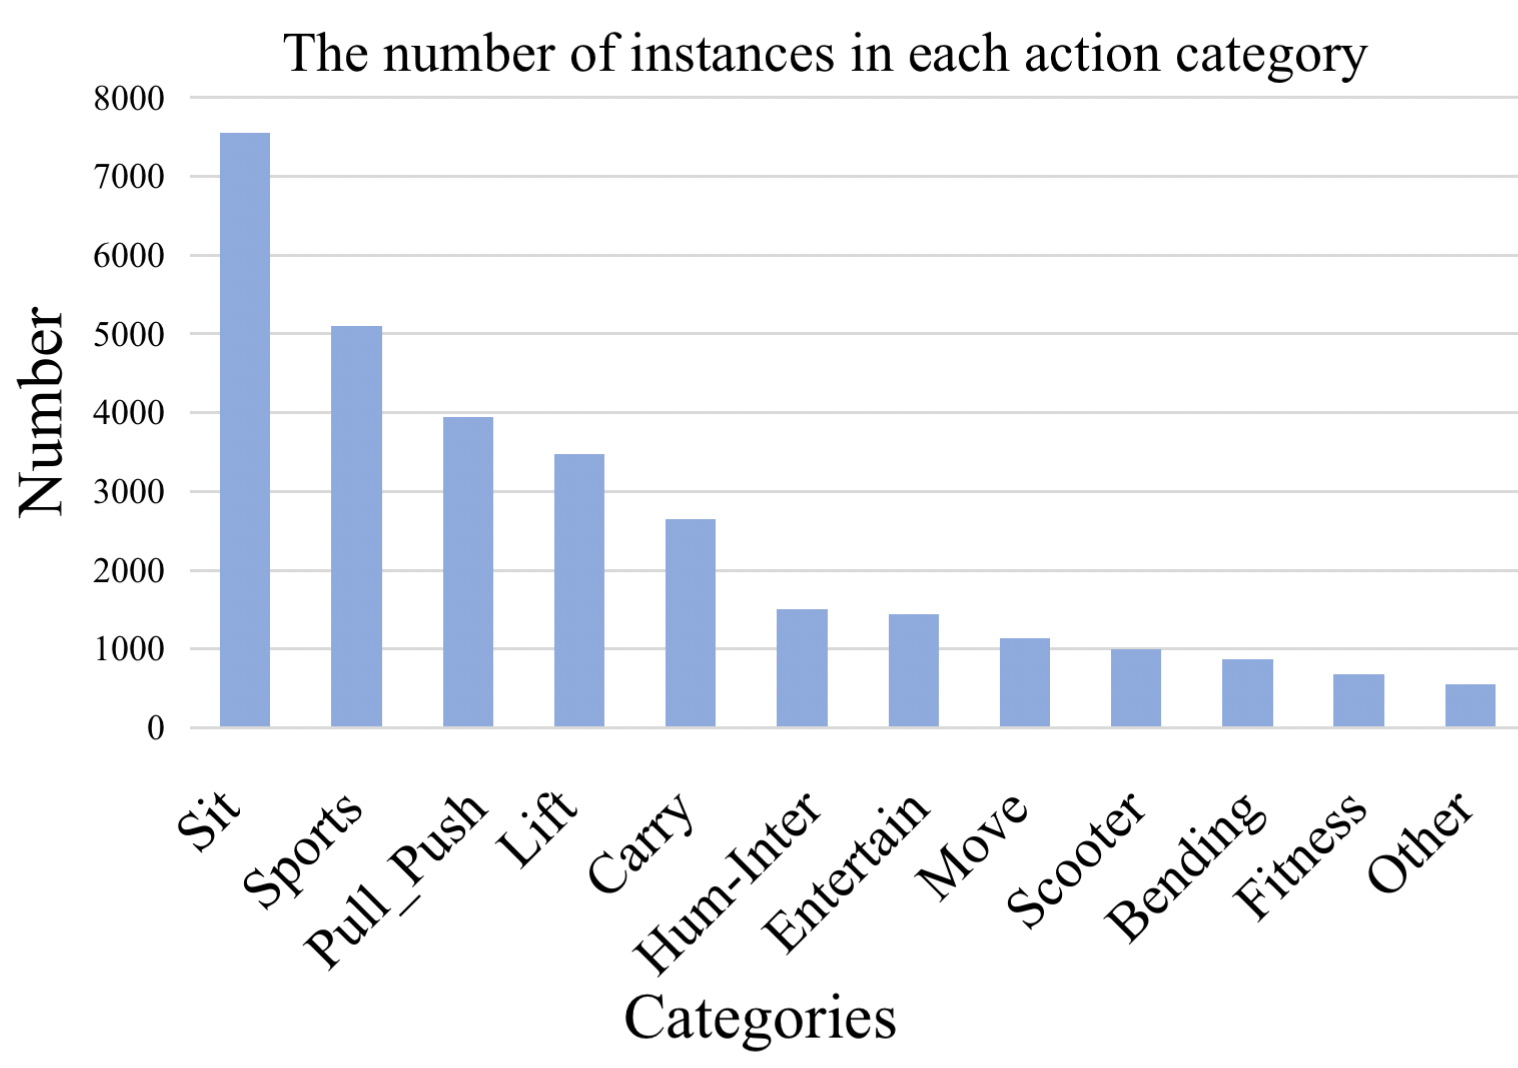
\includegraphics[width=0.93\columnwidth]{sup-pic/actioncount.png}
    \caption{The number of instance in each merged action category.}
    \label{fig:action_count}
    \vspace{-2ex}
\end{figure}




% Please add the following required packages to your document preamble:
% \usepackage{multirow}
\begin{table}[ht]
\caption{Detailed action priority and merge information.}
\centering
\label{tab:action_merge}
\resizebox{0.85\linewidth}{!}{   
\begin{tabular}{l|c|l}
\hline
Merged   Action                      & priority            & Original Action                    \\ \hline
\multirow{7}{*}{Lift}                & \multirow{7}{*}{0}  & taking clothes                     \\ \cline{3-3} 
                                     &                     & lifting a   plastic bag            \\ \cline{3-3} 
                                     &                     & lifting a bag                      \\ \cline{3-3} 
                                     &                     & taking   things/exchanging items   \\ \cline{3-3} 
                                     &                     & lifting   things                   \\ \cline{3-3} 
                                     &                     & lifting something                  \\ \cline{3-3} 
                                     &                     & moving planks                      \\ \hline
\multirow{3}{*}{Carry}               & \multirow{3}{*}{1}  & carrying other things              \\ \cline{3-3} 
                                     &                     & carrying a bag                     \\ \cline{3-3} 
                                     &                     & carrying bags                      \\ \hline
Move                                 & 2                   & moving boxes                       \\ \hline
\multirow{10}{*}{Pull\_Push}          & \multirow{10}{*}{3} & pulling a suitcase                 \\ \cline{3-3} 
                                     &                     & pulling a chair                    \\ \cline{3-3} 
                                     &                     & pulling a flatcar                  \\ \cline{3-3} 
                                     &                     & pushing a cart                     \\ \cline{3-3} 
                                     &                     & pushing a stroller                 \\ \cline{3-3} 
                                     &                     & pushing a flatcar                  \\ \cline{3-3} 
                                     &                     & pushing a table                    \\ \cline{3-3} 
                                     &                     & holding a spring car               \\ \cline{3-3} 
                                     &                     & pushing something                  \\ \cline{3-3} 
                                     &                     & pushing something                  \\ \hline
\multirow{14}{*}{Sit}                & \multirow{5}{*}{4}  & riding a bicycle                   \\ \cline{3-3} 
                                     &                     & riding an electric bicycle         \\ \cline{3-3} 
                                     &                     & riding a tricycle                   \\ \cline{3-3} 
                                     &                     & riding on the carousel             \\ \cline{3-3} 
                                     &                     & sitting in a spring car            \\ \cline{2-3} 
                                     & \multirow{9}{*}{13} & crouching                          \\ \cline{3-3} 
                                     &                     & sitting on the ground              \\ \cline{3-3} 
                                     &                     & crouching or sitting on the ground \\ \cline{3-3} 
                                     &                     & sitting on the ground              \\ \cline{3-3} 
                                     &                     & sitting                            \\ \cline{3-3} 
                                     &                     & sitting on a trunk                 \\ \cline{3-3} 
                                     &                     & sitting in a chair                 \\ \cline{3-3} 
                                     &                     & sitting on the stool               \\ \cline{3-3} 
                                     &                     & squatting                          \\ \hline
\multirow{5}{*}{Scooter-BalanceBike} & \multirow{5}{*}{5}  & riding a two-wheel balance car     \\ \cline{3-3} 
                                     &                     & riding a balance car               \\ \cline{3-3} 
                                     &                     & riding an electric skateboard      \\ \cline{3-3} 
                                     &                     & riding a skateboard                \\ \cline{3-3} 
                                     &                     & standing on a trolley              \\ \hline
\multirow{8}{*}{Hum-Inter}           & \multirow{8}{*}{6}  & hugging                            \\ \cline{3-3} 
                                     &                     & pulling a baby                     \\ \cline{3-3} 
                                     &                     & being hold by someone else         \\ \cline{3-3} 
                                     &                     & taking a baby                      \\ \cline{3-3} 
                                     &                     & holding the baby                   \\ \cline{3-3} 
                                     &                     & Being held by someone else         \\ \cline{3-3} 
                                     &                     & carrying a baby                    \\ \cline{3-3} 
                                     &                     & being carry by someone else        \\ \hline
\multirow{3}{*}{Fitness}             & \multirow{3}{*}{7}  & fitness with a twister             \\ \cline{3-3} 
                                     &                     & fitness with a elliptical trainer  \\ \cline{3-3} 
                                     &                     & fitness with a stepper             \\ \hline
\multirow{6}{*}{Entertain}           & \multirow{6}{*}{8}  & climbing the swing                 \\ \cline{3-3} 
                                     &                     & climbing slide                     \\ \cline{3-3} 
                                     &                     & holding the slide                  \\ \cline{3-3} 
                                     &                     & sliding                            \\ \cline{3-3} 
                                     &                     & playing seesaw                     \\ \cline{3-3} 
                                     &                     & sitting in a cavern                \\ \hline
\multirow{2}{*}{Sports}              & 9                   & playing basketball                 \\ \cline{2-3} 
                                     & 10                  & playing badminton                  \\ \hline
\multirow{5}{*}{Standing}            & 11                  & taking the escalator               \\ \cline{2-3} 
                                     & 14                  & running                            \\ \cline{2-3} 
                                     & \multirow{3}{*}{15} & walking                            \\ \cline{3-3} 
                                     &                     & standing                           \\ \cline{3-3} 
                                     &                     & leaning                            \\ \hline
Bending$\_$Over                         & 12                  & bending over                       \\ \hline
\multirow{8}{*}{Other}               & \multirow{8}{*}{16} & cabinet interaction                \\ \cline{3-3} 
                                     &                     & standing on the stool              \\ \cline{3-3} 
                                     &                     & getting in the car                 \\ \cline{3-3} 
                                     &                     & getting out of the car             \\ \cline{3-3} 
                                     &                     & driving a toy car                  \\ \cline{3-3} 
                                     &                     & lying                              \\ \cline{3-3} 
                                     &                     & writing on the blackboard          \\ \cline{3-3} 
                                     &                     & …                                  \\ \hline
\end{tabular}
}
\end{table}




\section{More Experiment}
We take pre-trained CenterPoint as the 3D Detector and add a feature extractor for cropped individual point cloud for the second-stage action recognition comparison, the detailed comparison result is shown in Table ~\ref{tab:action_exp1}. Our method outperforms others in most of categories. The comparison result which uses 3D bounding boxes from ground truth is shown in Table ~\ref{tab:action_abcde_ground}. We further provide
action visualization in Figure ~\ref{fig:vis-action}.
% \begin{wrapfigure}{r}{3.5cm}
\begin{figure}[ht]

    \centering

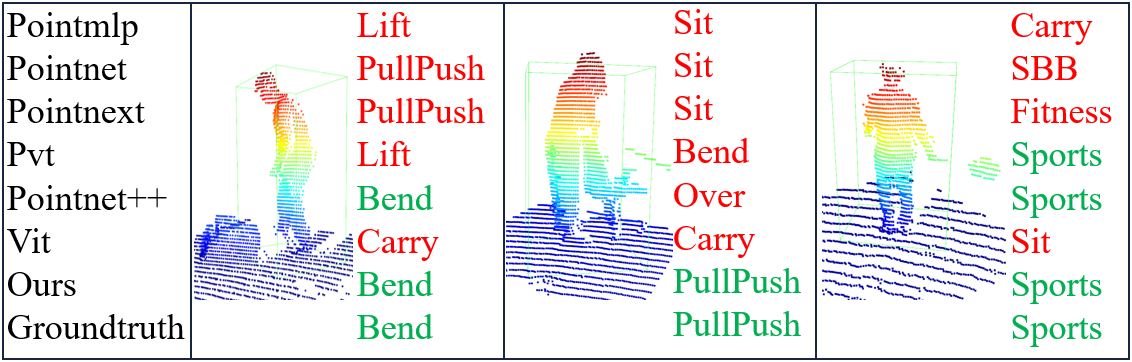
\includegraphics[width=1\columnwidth]{pic/rebuttalimg3.jpg}
   % \caption{Visualization for action recognition. SBB denotes the class Scooter-BalanceBike, the words in green are the correct prediction and the red are the wrong predictions.}
    \label{fig:vis-action}
\end{figure}

\begin{table*}[ht]
\caption{Detailed comparison results of action recognition on HuCenLife. All methods are based on the same 3D detector (centerpoint) for fair evaluation.}
\label{tab:action_exp1}

\setlength{\tabcolsep}{1.3mm}
\resizebox{\linewidth}{!}{     
\begin{tabular}{c|c|c|c|c|c|c|c|c|c|c|c|c|c|c|c}
\hline
Method           & Lift         & Carry         & Move         & Pull\_Push     & Sit           & Scooter-BalanceBike & Hum-Inter    & Fitness       & Entertain     & Sports        & Bend-Over    & Standing      & mAP         & mRecall     & mPrec         \\ \hline
Baseline         & 0.5          & 1.6           & 0.2           & 13.8          & 2.2           & 21.8                & 0            & 0             & 2.4           & 6.9           & 0.1          & \textbf{38.3} & 7.3         & 14.6        & 19.9          \\ \hline
ViT              & 4.1          & 1.6           & 5.1           & 8.2           & 0.6           & 4.7                 & 0.1          & \textbf{27.3} & 6             & \textbf{46.6} & 0.1          & 8.3           & 9.4         & 23.1        & 19.9          \\ \hline
PVT              & 1.4          & 10.5          & 8.9           & 21            & 16.8          & 56.8                & 5.9          & 1.7           & 1             & 25.1          & 4.3          & 5.2           & 13.2        & 30.5        & 19.8          \\ \hline
PointNet         & 1.6          & 3.1           & 4.6           & 20.1          & 24.4          & 22.3                & 0.7          & 0.6           & 0.6           & 17.1          & 1.5          & 4.2           & 8.4         & 26.3        & 15.5          \\ \hline
PointNet++       & 3.6          & 25.3          & 10.6          & 21            & 25.5          & 51                  & 3.5          & 2.7           & 3.3           & 30.3          & 4.1          & 6.5           & 15.6        & 34.2        & 22.7          \\ \hline
PointMLP         & 2.9          & 4.1           & 7.6           & 24.6          & 23.6          & 34.4                & 2.8          & 1.8           & 2.7           & 25.4          & 1.6          & 3.9           & 11.3        & 28          & 19.4          \\ \hline
PointNeXt        & 2            & 13.3          & 15.2          & 26.1          & 12.8          & 61.1                & 5.4          & 4.7           & 1.7           & 26.6          & 3.2          & 8.4           & 15          & 33          & 21.2          \\ \hline
Ours             & 5            & \textbf{26.5} & \textbf{20.1} & \textbf{35.8} & \textbf{26.5} & \textbf{68.5}       & 6.8          & 6.2           & \textbf{11.2} & 30.4          & 4.5          & 10.8          & \textbf{21} & \textbf{40} & \textbf{26.9} \\ \hline
Ours(w/o   ENFI) & \textbf{6.1} & 16.7          & 16.8          & 31            & 18.4          & 55.8                & \textbf{7.8} & 3.9           & 1.3           & 11.7          & \textbf{4.6} & 10.9          & 15.4        & 37.1        & 24.7          \\ \hline
\end{tabular}
}
\end{table*}


\begin{table*}[ht]
\caption{Detailed comparison results of action recognition on HuCenLife. All methods are based on the ground truth bounding boxes. mAcc stands for mean accuracy.}
\label{tab:action_abcde_ground}

\setlength{\tabcolsep}{1.3mm}
\resizebox{\linewidth}{!}{     
\begin{tabular}{c|c|c|c|c|c|c|c|c|c|c|c|c|c}
\hline
Method         & Lift & Carry & Move & Pull\_Push & Sit  & Scooter-BalanceBike & Hum-Inter & Fitness & Entertain & Sports & Bend-Over & Standing & mAcc \\ \hline
ViT            & 9.1  & 10.7  & 26.2 & 36.3       & 25.3 & 15.2               & 1.9      & 51.6    & 50.9      & 65.5   & 13.5      & 16.0     & 26.9 \\ \hline
PVT            & 4.5  & 42.8  & 31.2 & 35.6       & 40.0 & 74.7               & 7.2      & 36.4    & 0.4       & 16.2   & 54.4      & 31.6     & 31.3 \\ \hline
PointNet       & 7.8  & 29.1  & 32.8 & 33.2       & 47.2 & 53.1               & 7.5      & 46.9    & 19.1      & 20.1   & 57.4      & 20.9     & 31.3 \\ \hline
PointNet++     & 11.1 & 41.1  & 37.7 & 23.5       & 66.7 & 80.3               & 15.5     & 39.3    & 55.4      & 11.4   & 30.3      & 8.6      & 35.1 \\ \hline
PointMLP       & 25.6 & 46.4  & 35.4 & 57.2       & 55.2 & 79.7               & 4.9      & 54.5    & 27.8      & 15.3   & 29.1      & 32.8     & 38.7 \\ \hline
PointNext      & 11.8 & 46.7  & 24.0 & 49.4       & 50.1 & 76.1               & 21.6     & 46.9    & 36.5      & 10.2   & 36.2      & 53.0     & 38.5 \\ \hline
Ours           & 19.8 & 38.9  & 30.0 & 59.8       & 62.5 & 86.6               & 62.5     & 61.8    & 32.4      & 18.2   & 35.0      & 24.8     & \textbf{44.4} \\ \hline
Ours(w/o ENFI) & 18.9 & 49.5  & 47.6 & 57.2       & 53.3 & 83.1               & 28.8     & 31.5    & 31.2      & 19.2   & 53.6      & 33.8     & 42.3 \\ \hline
               
\end{tabular}
}
\end{table*}

%-------------------------------------------------------------------------

% {\small
% \bibliographystyle{ieee_fullname}
% \bibliography{egbib}
% }

\end{appendix}

\end{document}